% Options for packages loaded elsewhere
\PassOptionsToPackage{unicode}{hyperref}
\PassOptionsToPackage{hyphens}{url}
\documentclass[
  11pt,
  fontset=fandol]{ctexart}
\usepackage{xcolor}
\usepackage[margin=2cm]{geometry}
\usepackage{amsmath,amssymb}
\setcounter{secnumdepth}{-\maxdimen} % remove section numbering
\usepackage{iftex}
\ifPDFTeX
  \usepackage[T1]{fontenc}
  \usepackage[utf8]{inputenc}
  \usepackage{textcomp} % provide euro and other symbols
\else % if luatex or xetex
  \usepackage{unicode-math} % this also loads fontspec
  \defaultfontfeatures{Scale=MatchLowercase}
  \defaultfontfeatures[\rmfamily]{Ligatures=TeX,Scale=1}
\fi
\usepackage{lmodern}
\ifPDFTeX\else
  % xetex/luatex font selection
\fi
% Use upquote if available, for straight quotes in verbatim environments
\IfFileExists{upquote.sty}{\usepackage{upquote}}{}
\IfFileExists{microtype.sty}{% use microtype if available
  \usepackage[]{microtype}
  \UseMicrotypeSet[protrusion]{basicmath} % disable protrusion for tt fonts
}{}
\makeatletter
\@ifundefined{KOMAClassName}{% if non-KOMA class
  \IfFileExists{parskip.sty}{%
    \usepackage{parskip}
  }{% else
    \setlength{\parindent}{0pt}
    \setlength{\parskip}{6pt plus 2pt minus 1pt}}
}{% if KOMA class
  \KOMAoptions{parskip=half}}
\makeatother
\usepackage{longtable,booktabs,array}
\usepackage{calc} % for calculating minipage widths
% Correct order of tables after \paragraph or \subparagraph
\usepackage{etoolbox}
\makeatletter
\patchcmd\longtable{\par}{\if@noskipsec\mbox{}\fi\par}{}{}
\makeatother
% Allow footnotes in longtable head/foot
\IfFileExists{footnotehyper.sty}{\usepackage{footnotehyper}}{\usepackage{footnote}}
\makesavenoteenv{longtable}
\setlength{\emergencystretch}{3em} % prevent overfull lines
\providecommand{\tightlist}{%
  \setlength{\itemsep}{0pt}\setlength{\parskip}{0pt}}
\usepackage{float}
\usepackage{caption}
\usepackage{tikz,pgfplots}
\usepackage{hyperref}
\pgfplotsset{compat=1.18}
\usepgfplotslibrary{groupplots}
\hypersetup{colorlinks=true,linkcolor=blue!50!black,urlcolor=blue!50!black}
\setlength{\emergencystretch}{3em}
\setlength{\parskip}{0.4em}
\pagestyle{plain}
\usepackage{bookmark}
\IfFileExists{xurl.sty}{\usepackage{xurl}}{} % add URL line breaks if available
\urlstyle{same}
\hypersetup{
  pdftitle={编码器更新位置与细胞核中心检测：P20--P29 阶段分析},
  hidelinks,
  pdfcreator={LaTeX via pandoc}}

\title{编码器更新位置与细胞核中心检测：P20--P29 阶段分析}
\author{}
\date{2026-11-15}

\begin{document}
\maketitle

{
\setcounter{tocdepth}{2}
\tableofcontents
}
P29 在原有十二层更新预算下，种子 19/1 分别多找到 16/13 个内部 Dead
类细胞核，总匹配增加 283/165，未匹配预测减少
65/64。两个配对图像重采样区间均为正，最终召回和精度仍低于原定绝对要求。四个模型均已完成
130 轮训练和开发评估。最后一项调度作业在保存阶段达到时间上限，随后 CPU
作业完整保存并核验了实验种子 1
的两个检查点与全部结果图片。结合本阶段各轮结果，改变编码器的更新范围，比已测试的额外类别监督、参数平均和预训练参数约束更稳定地改善了部分检测结果，但效果随层位置和组织图像而变化。

\subsection{数据角色与指标}\label{ux6570ux636eux89d2ux8272ux4e0eux6307ux6807}

每轮都从相同 UNI 预训练权重重新训练对照和实验模型，使用 PanNuke 第 1
折中的 2,134 张训练图像，并在同折预先留出的 522 张开发评估图像上评估第
130 轮检查点。总体召回以 12,250
个标注核为分母；精度以全部输出中心点为分母，包含未匹配预测。中心点与标注采用三原始像素半径的一对一匹配。模型输出一张不含类别标签的中心图，类别用于统计分层。

``内部 Dead''指 PanNuke
的凋亡或坏死核类别中，标注轮廓不接触图像边界的对象，共 11 张图像、145
个核；其中原始面积小于 67 像素的对象有 32 个。各轮保留种子
19/1、数据划分、解码规则、最后检查点和阈值。后续方案反复使用同一开发评估集，表中的变化均来自同轮新训练对照。实例分割的官方
PQ 和三划分评估另有独立协议。

下一轮 P30 在完整 P29 种子 1 结果出现前冻结，依据 P20--P28 的证据和 P29
的运行进度，比较中间十二层与最后十二层。P29 沿原作业继续运行。P30
的验收与正式提交见 \href{../P30_SUBMISSION.md}{P30\_SUBMISSION.md}。

\subsection{本阶段十项比较的研究意义}\label{ux672cux9636ux6bb5ux5341ux9879ux6bd4ux8f83ux7684ux7814ux7a76ux610fux4e49}

\begin{figure}[H]\centering
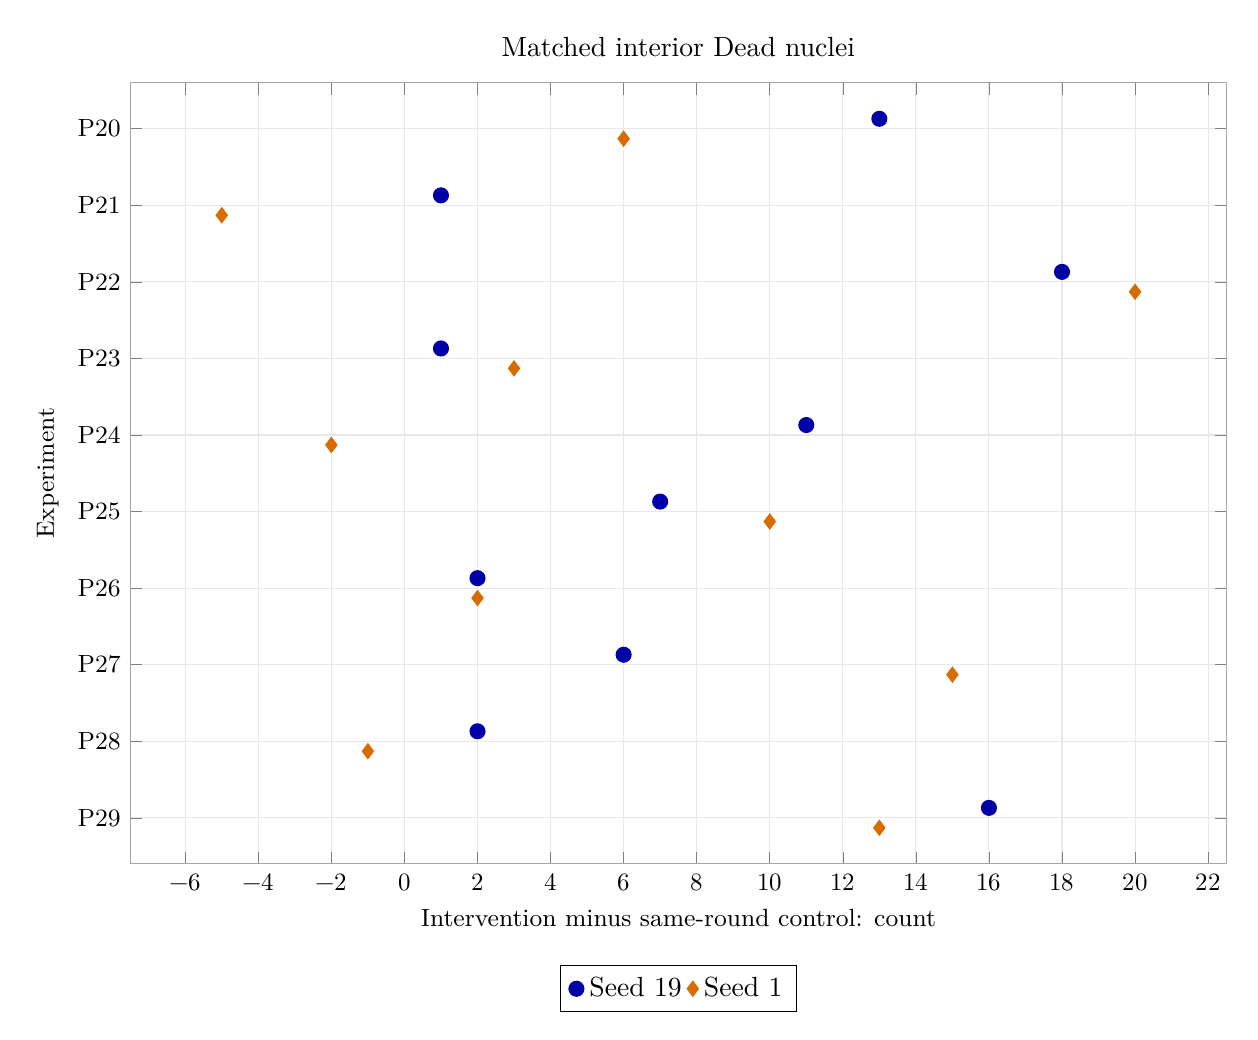
\begin{tikzpicture}
\begin{axis}[width=15.5cm,height=11.5cm,xlabel={Intervention minus same-round control: count},ylabel={Experiment},title={Matched interior Dead nuclei},ytick={0,1,2,3,4,5,6,7,8,9},yticklabels={P20,P21,P22,P23,P24,P25,P26,P27,P28,P29},ymin=-.6,ymax=9.6,y dir=reverse,grid=major,grid style={gray!18},legend style={at={(.5,-.13)},anchor=north,legend columns=2},axis line style={gray!70},tick label style={font=\small},label style={font=\small},title style={font=\normalsize}]
\addplot[only marks,mark=*,mark size=2.7pt,color=blue!65!black] coordinates {(13,-0.13) (1,0.87) (18,1.87) (1,2.87) (11,3.87) (7,4.87) (2,5.87) (6,6.87) (2,7.87) (16,8.87)};
\addlegendentry{Seed 19}
\addplot[only marks,mark=diamond*,mark size=2.7pt,color=orange!85!black] coordinates {(6,0.13) (-5,1.13) (20,2.13) (3,3.13) (-2,4.13) (10,5.13) (2,6.13) (15,7.13) (-1,8.13) (13,9.13)};
\addlegendentry{Seed 1}
\end{axis}
\end{tikzpicture}

\caption{各轮内部 Dead 匹配变化}
\end{figure}

\begin{figure}[H]\centering
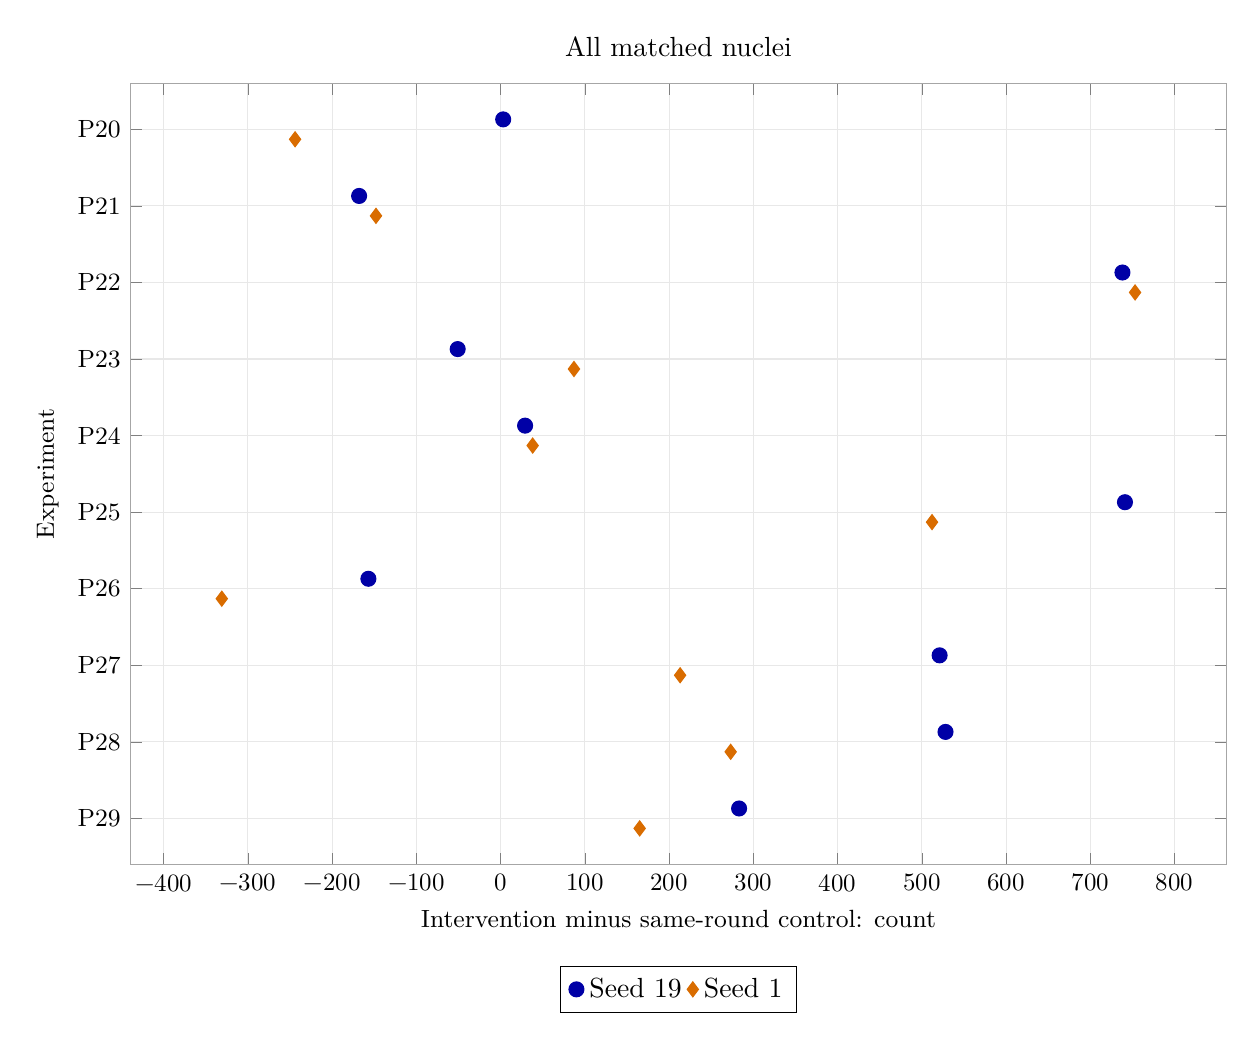
\begin{tikzpicture}
\begin{axis}[width=15.5cm,height=11.5cm,xlabel={Intervention minus same-round control: count},ylabel={Experiment},title={All matched nuclei},ytick={0,1,2,3,4,5,6,7,8,9},yticklabels={P20,P21,P22,P23,P24,P25,P26,P27,P28,P29},ymin=-.6,ymax=9.6,y dir=reverse,grid=major,grid style={gray!18},legend style={at={(.5,-.13)},anchor=north,legend columns=2},axis line style={gray!70},tick label style={font=\small},label style={font=\small},title style={font=\normalsize}]
\addplot[only marks,mark=*,mark size=2.7pt,color=blue!65!black] coordinates {(3,-0.13) (-168,0.87) (738,1.87) (-51,2.87) (29,3.87) (741,4.87) (-157,5.87) (521,6.87) (528,7.87) (283,8.87)};
\addlegendentry{Seed 19}
\addplot[only marks,mark=diamond*,mark size=2.7pt,color=orange!85!black] coordinates {(-244,0.13) (-148,1.13) (753,2.13) (87,3.13) (38,4.13) (512,5.13) (-331,6.13) (213,7.13) (273,8.13) (165,9.13)};
\addlegendentry{Seed 1}
\end{axis}
\end{tikzpicture}

\caption{各轮全部细胞核匹配变化}
\end{figure}

\begin{figure}[H]\centering
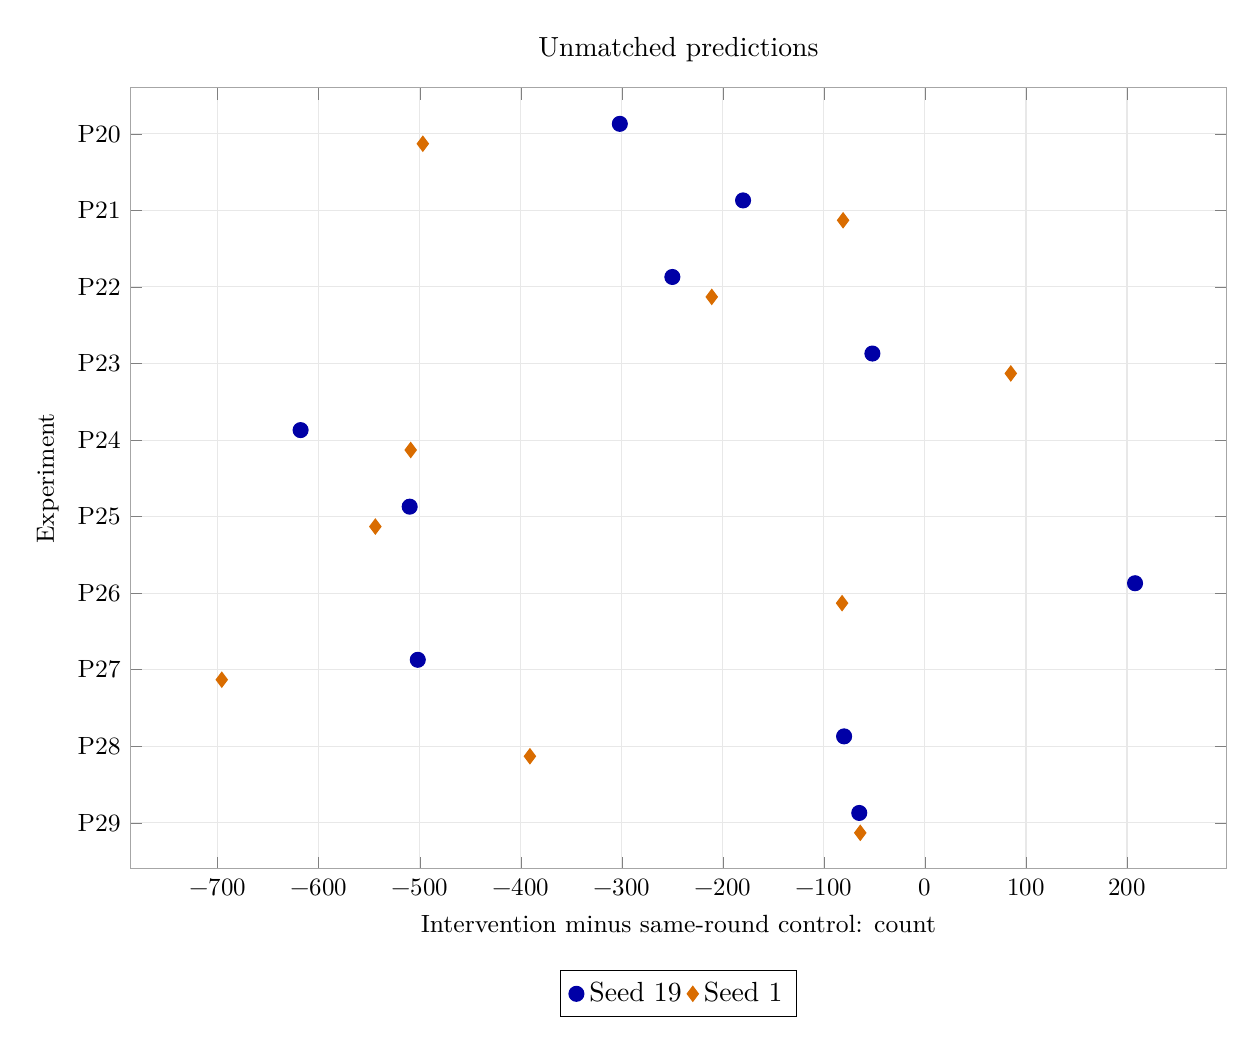
\begin{tikzpicture}
\begin{axis}[width=15.5cm,height=11.5cm,xlabel={Intervention minus same-round control: count},ylabel={Experiment},title={Unmatched predictions},ytick={0,1,2,3,4,5,6,7,8,9},yticklabels={P20,P21,P22,P23,P24,P25,P26,P27,P28,P29},ymin=-.6,ymax=9.6,y dir=reverse,grid=major,grid style={gray!18},legend style={at={(.5,-.13)},anchor=north,legend columns=2},axis line style={gray!70},tick label style={font=\small},label style={font=\small},title style={font=\normalsize}]
\addplot[only marks,mark=*,mark size=2.7pt,color=blue!65!black] coordinates {(-302,-0.13) (-180,0.87) (-250,1.87) (-52,2.87) (-618,3.87) (-510,4.87) (208,5.87) (-502,6.87) (-80,7.87) (-65,8.87)};
\addlegendentry{Seed 19}
\addplot[only marks,mark=diamond*,mark size=2.7pt,color=orange!85!black] coordinates {(-497,0.13) (-81,1.13) (-211,2.13) (85,3.13) (-509,4.13) (-544,5.13) (-82,6.13) (-696,7.13) (-391,8.13) (-64,9.13)};
\addlegendentry{Seed 1}
\end{axis}
\end{tikzpicture}

\caption{各轮未匹配预测变化}
\end{figure}

\begin{longtable}[]{@{}lrrr@{}}
\toprule\noalign{}
测试变化 & 内部 Dead 匹配，种子 19 / 1 & 总匹配 & 未匹配预测 \\
\midrule\noalign{}
\endhead
\bottomrule\noalign{}
\endlastfoot
输入扩大至 512，P20 & +13 / +6 & +3 / −244 & −302 / −497 \\
增加类别中心监督，P21 & +1 / −5 & −168 / −148 & −180 / −81 \\
更新全部 24 层，P22 & +18 / +20 & +738 / +753 & −250 / −211 \\
参数平均，P23 & +1 / +3 & −51 / +87 & −52 / +85 \\
提高后十二层学习率，P24 & +11 / −2 & +29 / +38 & −618 / −509 \\
全层分层学习率，P25 & +7 / +10 & +741 / +512 & −510 / −544 \\
预训练参数约束，P26 & +2 / +2 & −157 / −331 & +208 / −82 \\
更新前十二层，P27 & +6 / +15 & +521 / +213 & −502 / −696 \\
更新交错十二层，P28 & +2 / −1 & +528 / +273 & −80 / −391 \\
更新前六层和后六层，P29 & +16 / +13 & +283 / +165 & −65 / −64 \\
\end{longtable}

P20 通过更大的输入找回更多 Dead
核，但总体覆盖变化不一致，训练时间约为对照的 4.3
倍。它显示分辨率能影响目标对象的可检测性，同时带来明显成本。P21
使预测和真匹配一起减少，额外类别中心监督在这一固定损失下未改善稀有核的迁移。P23
的参数平均只改变少量 Dead 匹配，总体覆盖方向不一致。P24
删除了许多未匹配点，提高精度，但 Dead
改善在两个种子中反向。上述结果说明，减少预测和找回漏检是不同的研究目标。

P22 是本阶段最稳定的稀有类改善：多匹配 18/20 个内部 Dead 核和 738/753
个总核，同时减少额外点。其最终 Dead 召回为 58.62\%/56.55\%，精度为
72.84\%/73.36\%，完整编码器适配改善了当前开发检测，但仍未达到原定绝对条件。P25
也提高总体覆盖与精度，不过 Dead 只增加 7/10 个，而且肺组织增加 9/8
个、结肠减少 7/6 个。总体匹配变好，并未使目标类别在不同组织中一致改善。

P26 将参数约束在预训练值附近，总匹配减少 157/331，Dead
各增加两个，未复现全层更新的改善。P27
在与后十二层对照相同的可训练参数量下，增加 6/15 个 Dead 匹配、减少
502/696 个未匹配点，训练召回却降至 88.80\%/87.82\%。P28
把更新分散到交错层，训练召回恢复到约 96.3\%，Dead 改善则减弱为
+2/−1。P29 种子 19 的训练召回为 95.47\%，Dead 增加 16
个。更新位置因此是有实验依据的研究变量；训练集覆盖、参数量和更新层的分散程度都只能解释部分现象，表征机制仍需直接测量。

\subsection{P29 种子 19
的覆盖、精度与成本}\label{p29-ux79cdux5b50-19-ux7684ux8986ux76d6ux7cbeux5ea6ux4e0eux6210ux672c}

\begin{longtable}[]{@{}
  >{\raggedright\arraybackslash}p{(\linewidth - 12\tabcolsep) * \real{0.1111}}
  >{\raggedleft\arraybackslash}p{(\linewidth - 12\tabcolsep) * \real{0.1481}}
  >{\raggedleft\arraybackslash}p{(\linewidth - 12\tabcolsep) * \real{0.1481}}
  >{\raggedleft\arraybackslash}p{(\linewidth - 12\tabcolsep) * \real{0.1481}}
  >{\raggedleft\arraybackslash}p{(\linewidth - 12\tabcolsep) * \real{0.1481}}
  >{\raggedleft\arraybackslash}p{(\linewidth - 12\tabcolsep) * \real{0.1481}}
  >{\raggedleft\arraybackslash}p{(\linewidth - 12\tabcolsep) * \real{0.1481}}@{}}
\toprule\noalign{}
\begin{minipage}[b]{\linewidth}\raggedright
更新范围
\end{minipage} & \begin{minipage}[b]{\linewidth}\raggedleft
内部 Dead
\end{minipage} & \begin{minipage}[b]{\linewidth}\raggedleft
小 Dead
\end{minipage} & \begin{minipage}[b]{\linewidth}\raggedleft
全部匹配
\end{minipage} & \begin{minipage}[b]{\linewidth}\raggedleft
总召回
\end{minipage} & \begin{minipage}[b]{\linewidth}\raggedleft
精度
\end{minipage} & \begin{minipage}[b]{\linewidth}\raggedleft
未匹配预测
\end{minipage} \\
\midrule\noalign{}
\endhead
\bottomrule\noalign{}
\endlastfoot
最后十二层 & 65/145 & 7/32 & 7,257/12,250 & 59.24\% & 69.73\% & 3,150 \\
前六层＋后六层 & 81/145 & 11/32 & 7,540/12,250 & 61.55\% & 70.96\% &
3,085 \\
\end{longtable}

实验模型多输出 218 个点，却多匹配 283 个核，预测的有效性有所提高。内部
Dead 召回增加 11.0345 个百分点，原固定 1,000
次按组织分层的图像重采样区间为 ［+3.0457，+27.9570］个百分点；总召回增加
2.3102 个百分点、精度增加 1.2328 个百分点。原种子级完整条件中，绝对 Dead
召回 0.60 和精度 0.75 两项未满足，其余种子 19 条件均满足。种子 1 的内部
Dead 召回改善为 8.9655 个百分点，同样未满足两项绝对条件。

训练集总体召回从 97.51\% 降至 95.47\%，训练内部 Dead 覆盖从 630/656 降至
607/656。纯训练时间为 4.0130/4.8652 小时，实验模型增加约
21.24\%；峰值已分配显存约为 4.05/4.84 GiB。种子 19 两项调度总耗时分别为
4:13:24 和
5:00:21，包含启动、评估和保存。训练覆盖、开发检测和调度成本分别回答不同的问题。

\begin{figure}[H]\centering
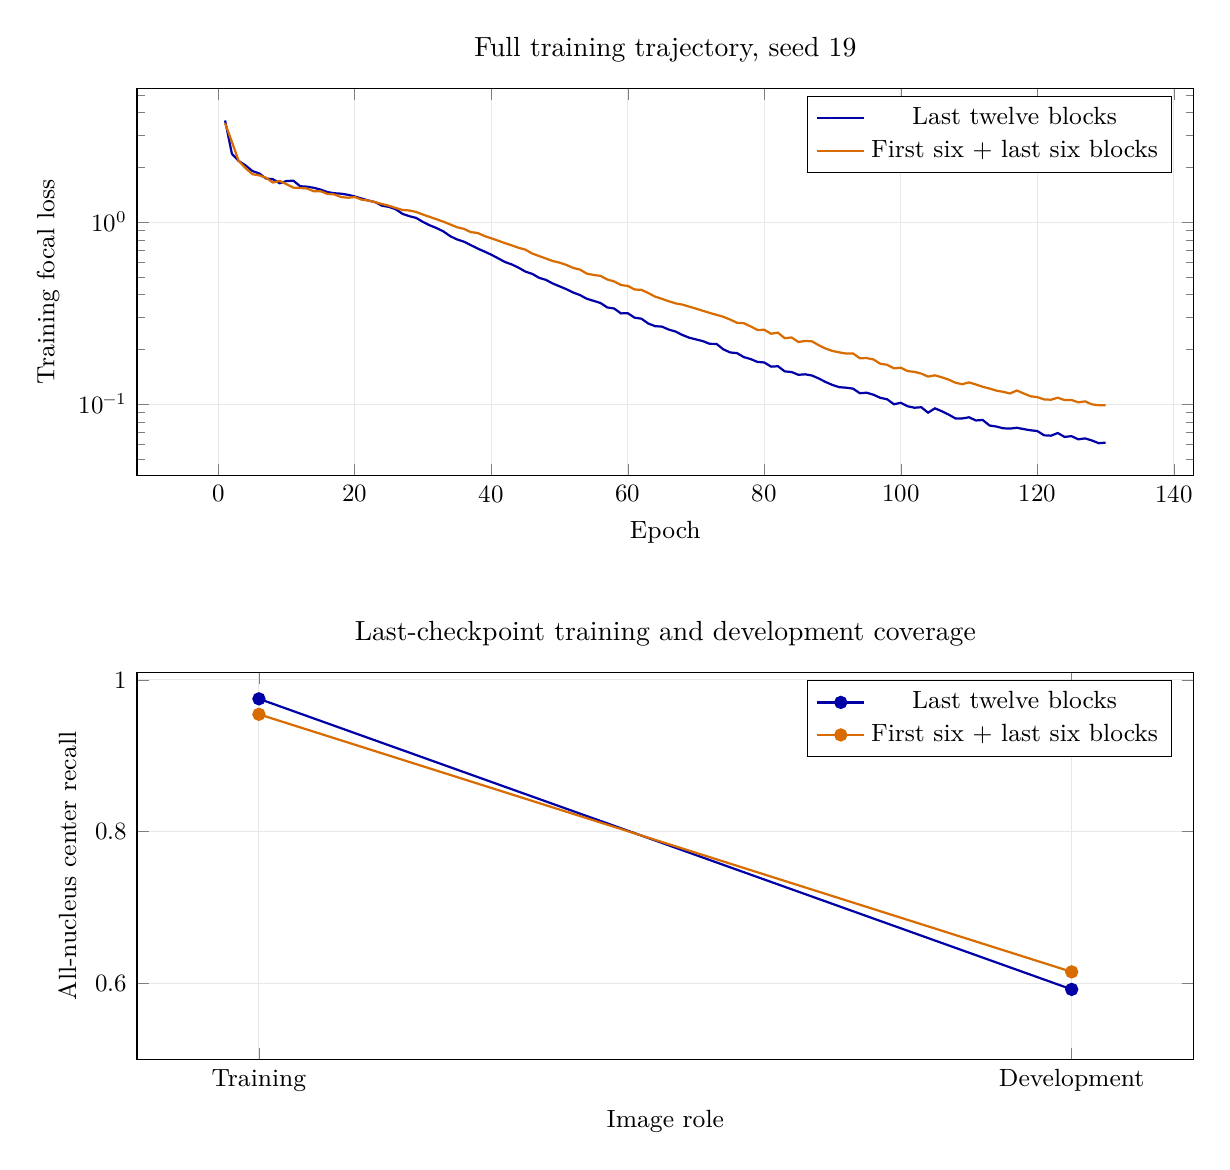
\begin{tikzpicture}
\begin{groupplot}[group style={group size=1 by 2,vertical sep=2.5cm},width=15cm,height=6.5cm,grid=major,grid style={gray!18},legend style={font=\small},tick label style={font=\small},label style={font=\small},title style={font=\normalsize}]
\nextgroupplot[xlabel={Epoch},ylabel={Training focal loss},ymode=log,title={Full training trajectory, seed 19}]
\addplot[thick,color=blue!65!black] coordinates {(1,3.62386978209) (2,2.37552843165) (3,2.1699790582) (4,2.05083011871) (5,1.91124379869) (6,1.85306071716) (7,1.73830157976) (8,1.72317317723) (9,1.63716908066) (10,1.68299786846) (11,1.69219968882) (12,1.57655350178) (13,1.56793110214) (14,1.54554083125) (15,1.51068508564) (16,1.46400284926) (17,1.44252403023) (18,1.43446976444) (19,1.41490890473) (20,1.38527809719) (21,1.34936290868) (22,1.31520210644) (23,1.28915614926) (24,1.23129468712) (25,1.21430525547) (26,1.17777008382) (27,1.11140446291) (28,1.07907247314) (29,1.05578593797) (30,1.00256185944) (31,0.961115168291) (32,0.927977368473) (33,0.889346529835) (34,0.837489534103) (35,0.803761817047) (36,0.781447936886) (37,0.748062575356) (38,0.716612512178) (39,0.690093925696) (40,0.662901303416) (41,0.633349982007) (42,0.604437001957) (43,0.586148878439) (44,0.56240585762) (45,0.535049840808) (46,0.52007716346) (47,0.494900800501) (48,0.482175430491) (49,0.460473351715) (50,0.444158400534) (51,0.428483899194) (52,0.410752979311) (53,0.397682718374) (54,0.379469061984) (55,0.369665312337) (56,0.3597513164) (57,0.339892074871) (58,0.3355475312) (59,0.315381314616) (60,0.316084984617) (61,0.29880171501) (62,0.294916734044) (63,0.277473928217) (64,0.268344895773) (65,0.266779590272) (66,0.256976687361) (67,0.250711295104) (68,0.239990992582) (69,0.231839629632) (70,0.22687595172) (71,0.222037940652) (72,0.214563905512) (73,0.214325386403) (74,0.200130272068) (75,0.192422631313) (76,0.190850315003) (77,0.181378530923) (78,0.176991748792) (79,0.170684004576) (80,0.169478886474) (81,0.160782273263) (82,0.161583742678) (83,0.151403813556) (84,0.150206022232) (85,0.145022003989) (86,0.145890951062) (87,0.143605590676) (88,0.138312381576) (89,0.132313917474) (90,0.127416898005) (91,0.123964854301) (92,0.123164128256) (93,0.121683641281) (94,0.114873931265) (95,0.115586895261) (96,0.11267241873) (97,0.108353732171) (98,0.106374115275) (99,0.0999097410195) (100,0.101763770482) (101,0.0973861433292) (102,0.0956012586589) (103,0.0961770233598) (104,0.0898133710938) (105,0.0948688865752) (106,0.0914647224007) (107,0.0876876159738) (108,0.0835042551837) (109,0.0834624404777) (110,0.0847086207095) (111,0.081374704054) (112,0.0818419124579) (113,0.0763423845631) (114,0.0753366971919) (115,0.0736962775521) (116,0.073428697569) (117,0.0741943524436) (118,0.072946563604) (119,0.0718636737304) (120,0.0711843375659) (121,0.0674173853084) (122,0.0671176563974) (123,0.0693980144741) (124,0.0660580317782) (125,0.0667165935397) (126,0.0640829772725) (127,0.0648491781496) (128,0.0631586541985) (129,0.0610245662421) (130,0.0614443497449)};
\addlegendentry{Last twelve blocks}
\addplot[thick,color=orange!85!black] coordinates {(1,3.50105492356) (2,2.76289148384) (3,2.17038305907) (4,1.98312889879) (5,1.83590344865) (6,1.80892446338) (7,1.75439191267) (8,1.65186924516) (9,1.68502842514) (10,1.6174624693) (11,1.54911897966) (12,1.54232221831) (13,1.53134093183) (14,1.4787512504) (15,1.47922120177) (16,1.42957731283) (17,1.42129815264) (18,1.37443559306) (19,1.36327421378) (20,1.37542054736) (21,1.33016328574) (22,1.31518258203) (23,1.28756736924) (24,1.25844964483) (25,1.23172492314) (26,1.19774090467) (27,1.16697317507) (28,1.15981375325) (29,1.1382047245) (30,1.10121632304) (31,1.06901810135) (32,1.03754835332) (33,1.00610931113) (34,0.971616917315) (35,0.937913104096) (36,0.919036173231) (37,0.881783900411) (38,0.87277482538) (39,0.839935905931) (40,0.815554868329) (41,0.792132447564) (42,0.767330217063) (43,0.746182883663) (44,0.723307935652) (45,0.706632291631) (46,0.672832300026) (47,0.65200705931) (48,0.63159530658) (49,0.61198255419) (50,0.599476133104) (51,0.582289886012) (52,0.560812200321) (53,0.548834211698) (54,0.521759605494) (55,0.512614208503) (56,0.507201689686) (57,0.484308340912) (58,0.472578119371) (59,0.451809032474) (60,0.446398185728) (61,0.426876144423) (62,0.424710518125) (63,0.408310935512) (64,0.390026470253) (65,0.379042657953) (66,0.36809506068) (67,0.358036929659) (68,0.352404804322) (69,0.343642305939) (70,0.334936154565) (71,0.325884575944) (72,0.317293170609) (73,0.309748381034) (74,0.302111506041) (75,0.291821877321) (76,0.279997927729) (77,0.278499311239) (78,0.26754597844) (79,0.255842017163) (80,0.256262032252) (81,0.243800983989) (82,0.247128760941) (83,0.230332737019) (84,0.232489445869) (85,0.219672735791) (86,0.222537847046) (87,0.221399081085) (88,0.210550299569) (89,0.202055267706) (90,0.196092654535) (91,0.192539622031) (92,0.189735345935) (93,0.189959515611) (94,0.178786053381) (95,0.179221209236) (96,0.176041919675) (97,0.166773603559) (98,0.164553097721) (99,0.157313765623) (100,0.158646976891) (101,0.151932625451) (102,0.150512845719) (103,0.147210237615) (104,0.141779869506) (105,0.144020077068) (106,0.140556078439) (107,0.136488059869) (108,0.131228308264) (109,0.12870185654) (110,0.13169746431) (111,0.128227441007) (112,0.124542114723) (113,0.12187337539) (114,0.118651823402) (115,0.116943936811) (116,0.114445477206) (117,0.118868027916) (118,0.114558337975) (119,0.110518558363) (120,0.109255300938) (121,0.10619787934) (122,0.105784444191) (123,0.108507285318) (124,0.105264322801) (125,0.105468319092) (126,0.102285939834) (127,0.10359711623) (128,0.0997327014371) (129,0.0986843192636) (130,0.0987533847518)};
\addlegendentry{First six + last six blocks}
\nextgroupplot[xlabel={Image role},ylabel={All-nucleus center recall},title={Last-checkpoint training and development coverage},xtick={0,1},xticklabels={Training,Development},xmin=-.15,xmax=1.15,ymin=.5,ymax=1.01]
\addplot[thick,mark=*,color=blue!65!black] coordinates {(0,0.975082404646) (1,0.592408163265)};
\addlegendentry{Last twelve blocks}
\addplot[thick,mark=*,color=orange!85!black] coordinates {(0,0.954697064825) (1,0.615510204082)};
\addlegendentry{First six + last six blocks}
\end{groupplot}
\end{tikzpicture}

\caption{完整训练过程及最后检查点覆盖}
\end{figure}

\subsection{哪些组织图像贡献了改善}\label{ux54eaux4e9bux7ec4ux7ec7ux56feux50cfux8d21ux732eux4e86ux6539ux5584}

\begin{figure}[H]\centering
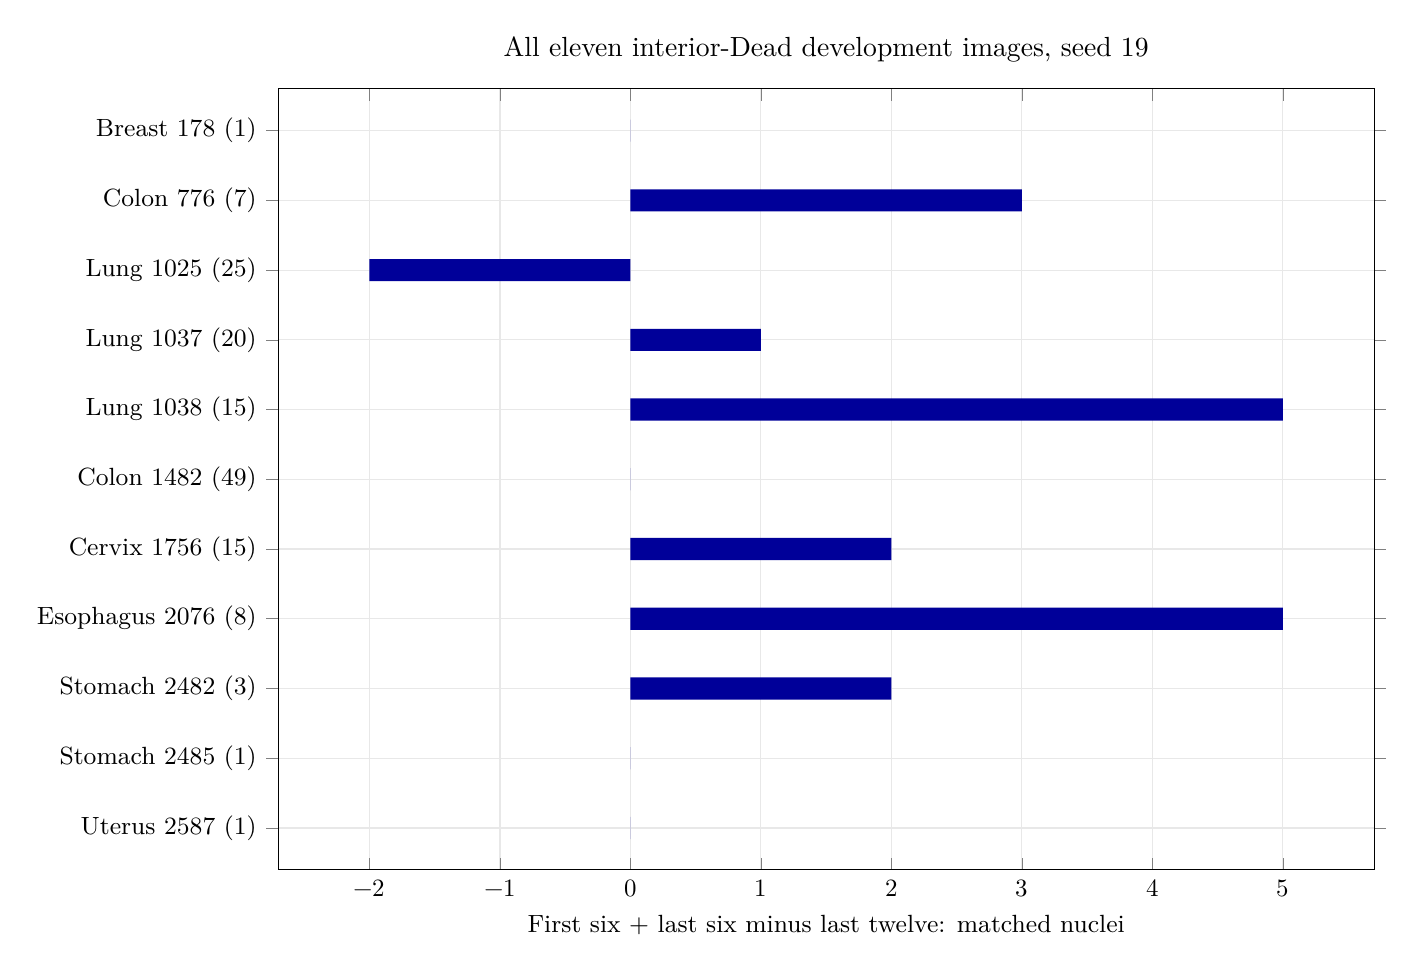
\begin{tikzpicture}
\begin{axis}[xbar,width=15.5cm,height=11.5cm,xlabel={First six + last six minus last twelve: matched nuclei},title={All eleven interior-Dead development images, seed 19},ytick={0,1,2,3,4,5,6,7,8,9,10},yticklabels={{Breast 178 (1)},{Colon 776 (7)},{Lung 1025 (25)},{Lung 1037 (20)},{Lung 1038 (15)},{Colon 1482 (49)},{Cervix 1756 (15)},{Esophagus 2076 (8)},{Stomach 2482 (3)},{Stomach 2485 (1)},{Uterus 2587 (1)}},ymin=-.6,ymax=10.6,y dir=reverse,bar width=8pt,grid=major,grid style={gray!18},tick label style={font=\small},label style={font=\small},title style={font=\normalsize}]
\addplot[fill=blue!60!black,draw=none] coordinates {(0,0) (3,1) (-2,2) (1,3) (5,4) (0,5) (2,6) (5,7) (2,8) (0,9) (0,10)};
\end{axis}
\end{tikzpicture}

\caption{包含内部 Dead 的全部十一张评估图像}
\end{figure}

六张图像增加匹配，一张减少，四张不变。肺组织净增加 4 个，结肠 3 个，宫颈
2 个，食管 5 个，胃 2 个；乳腺和子宫不变。肺组织图像 1038 和食管图像
2076 各增加 5 个，合计贡献 16 个净增量中的 10 个。肺组织图像 1025
则减少两个。结肠图像 1482 含 49/145 个目标对象，两臂均只匹配 13
个，该图仍有 36 个目标核未匹配。

逐一去掉一张 Dead 阳性图像作敏感性分析后，召回改善范围为
8.03\%--16.67\%，均为正。种子 19
的改善符号因此不依赖单张图像。正式原判定仍包含全部十一张图像。只有一张阳性图像的组织，提供的组织内跨图像一致性证据有限。

\subsection{固定样例中的逐核变化}\label{ux56faux5b9aux6837ux4f8bux4e2dux7684ux9010ux6838ux53d8ux5316}

预先固定的八张评估样例包含 53 个内部 Dead 核。种子 19 中，两臂共同找到
30 个，实验模型新增 6 个、丢失 4 个，共同漏检 13 个，净增两个；完整 522
张评估图像的净增量为 16。对象编号和行、列坐标保存在
\href{../fixed_objects.csv}{fixed\_objects.csv}。青色十字是预测点；白、绿、橙、粉色圆圈依次表示共同找到、新增、丢失和共同漏检。

\noindent

\begin{minipage}{\linewidth}\centering
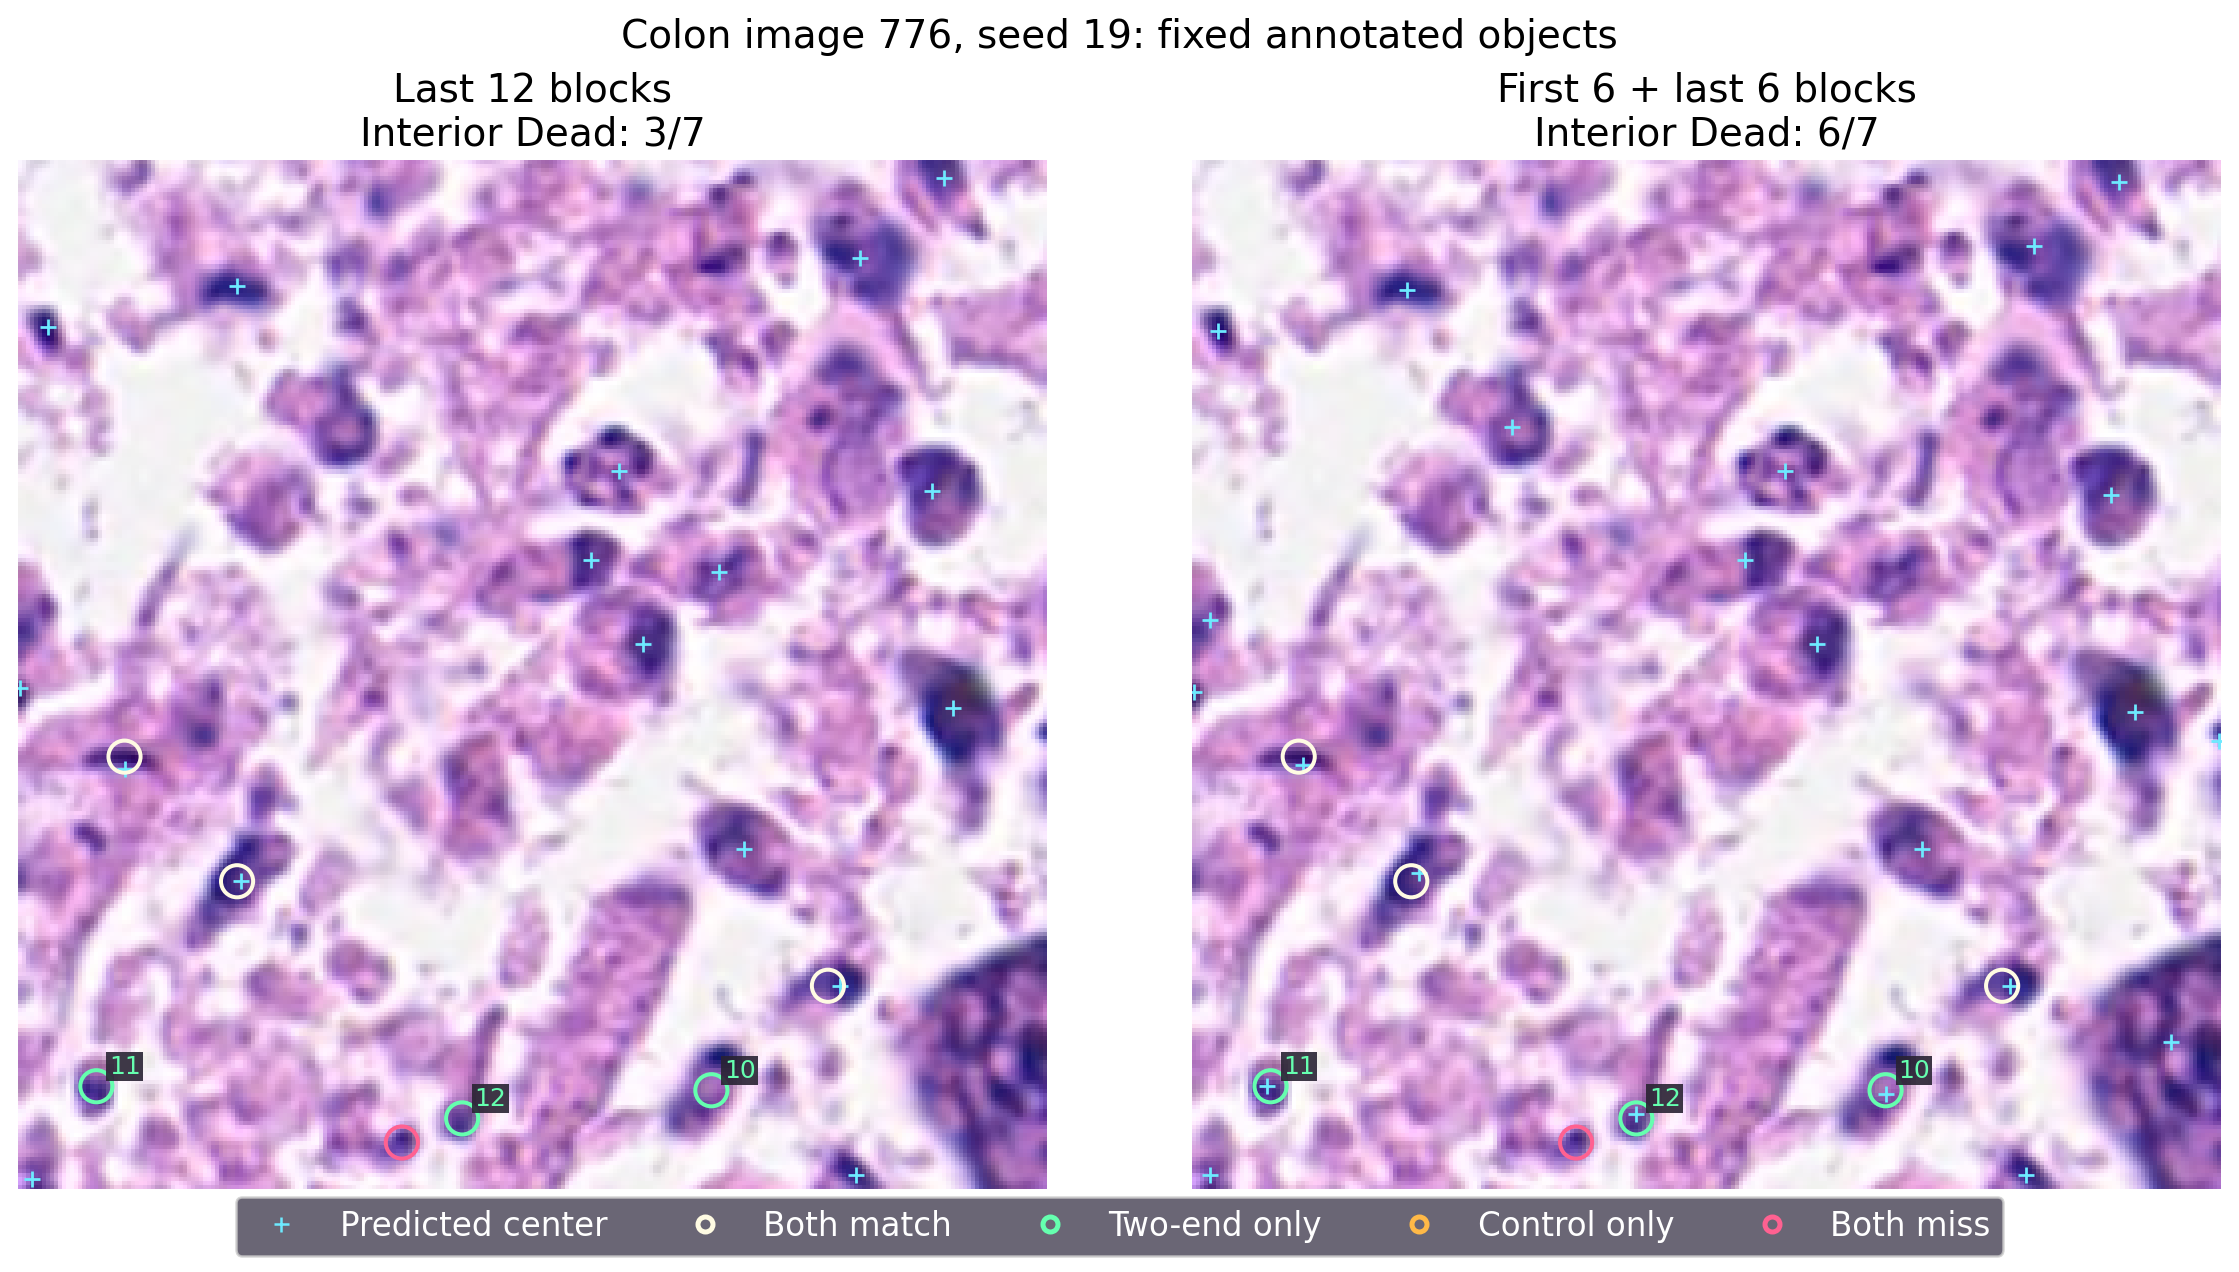
\includegraphics[width=\linewidth,height=0.40\textheight,keepaspectratio]{../figures/p29_image_776_seed_19.png}
\captionof{figure}{结肠图像 776：下方组织区域新增三个核}
\raggedright

结肠图像 776 的目标匹配从 3/7 升至 6/7。下方组织带中的对象 10 位于（231，172），对象 11 位于（230，19），对象 12 位于（238，110）；最近预测点距离分别从 41.23、28.02 和 80.66 像素降至 1.00 像素。右图在三个标注附近均出现预测，左图相应邻域缺少输出。这些核的可见大小和染色深浅不同，对象 12 面积为 104 像素，恢复对象覆盖了预定义最小面积组以外的核。

\end{minipage}

\noindent

\begin{minipage}{\linewidth}\centering
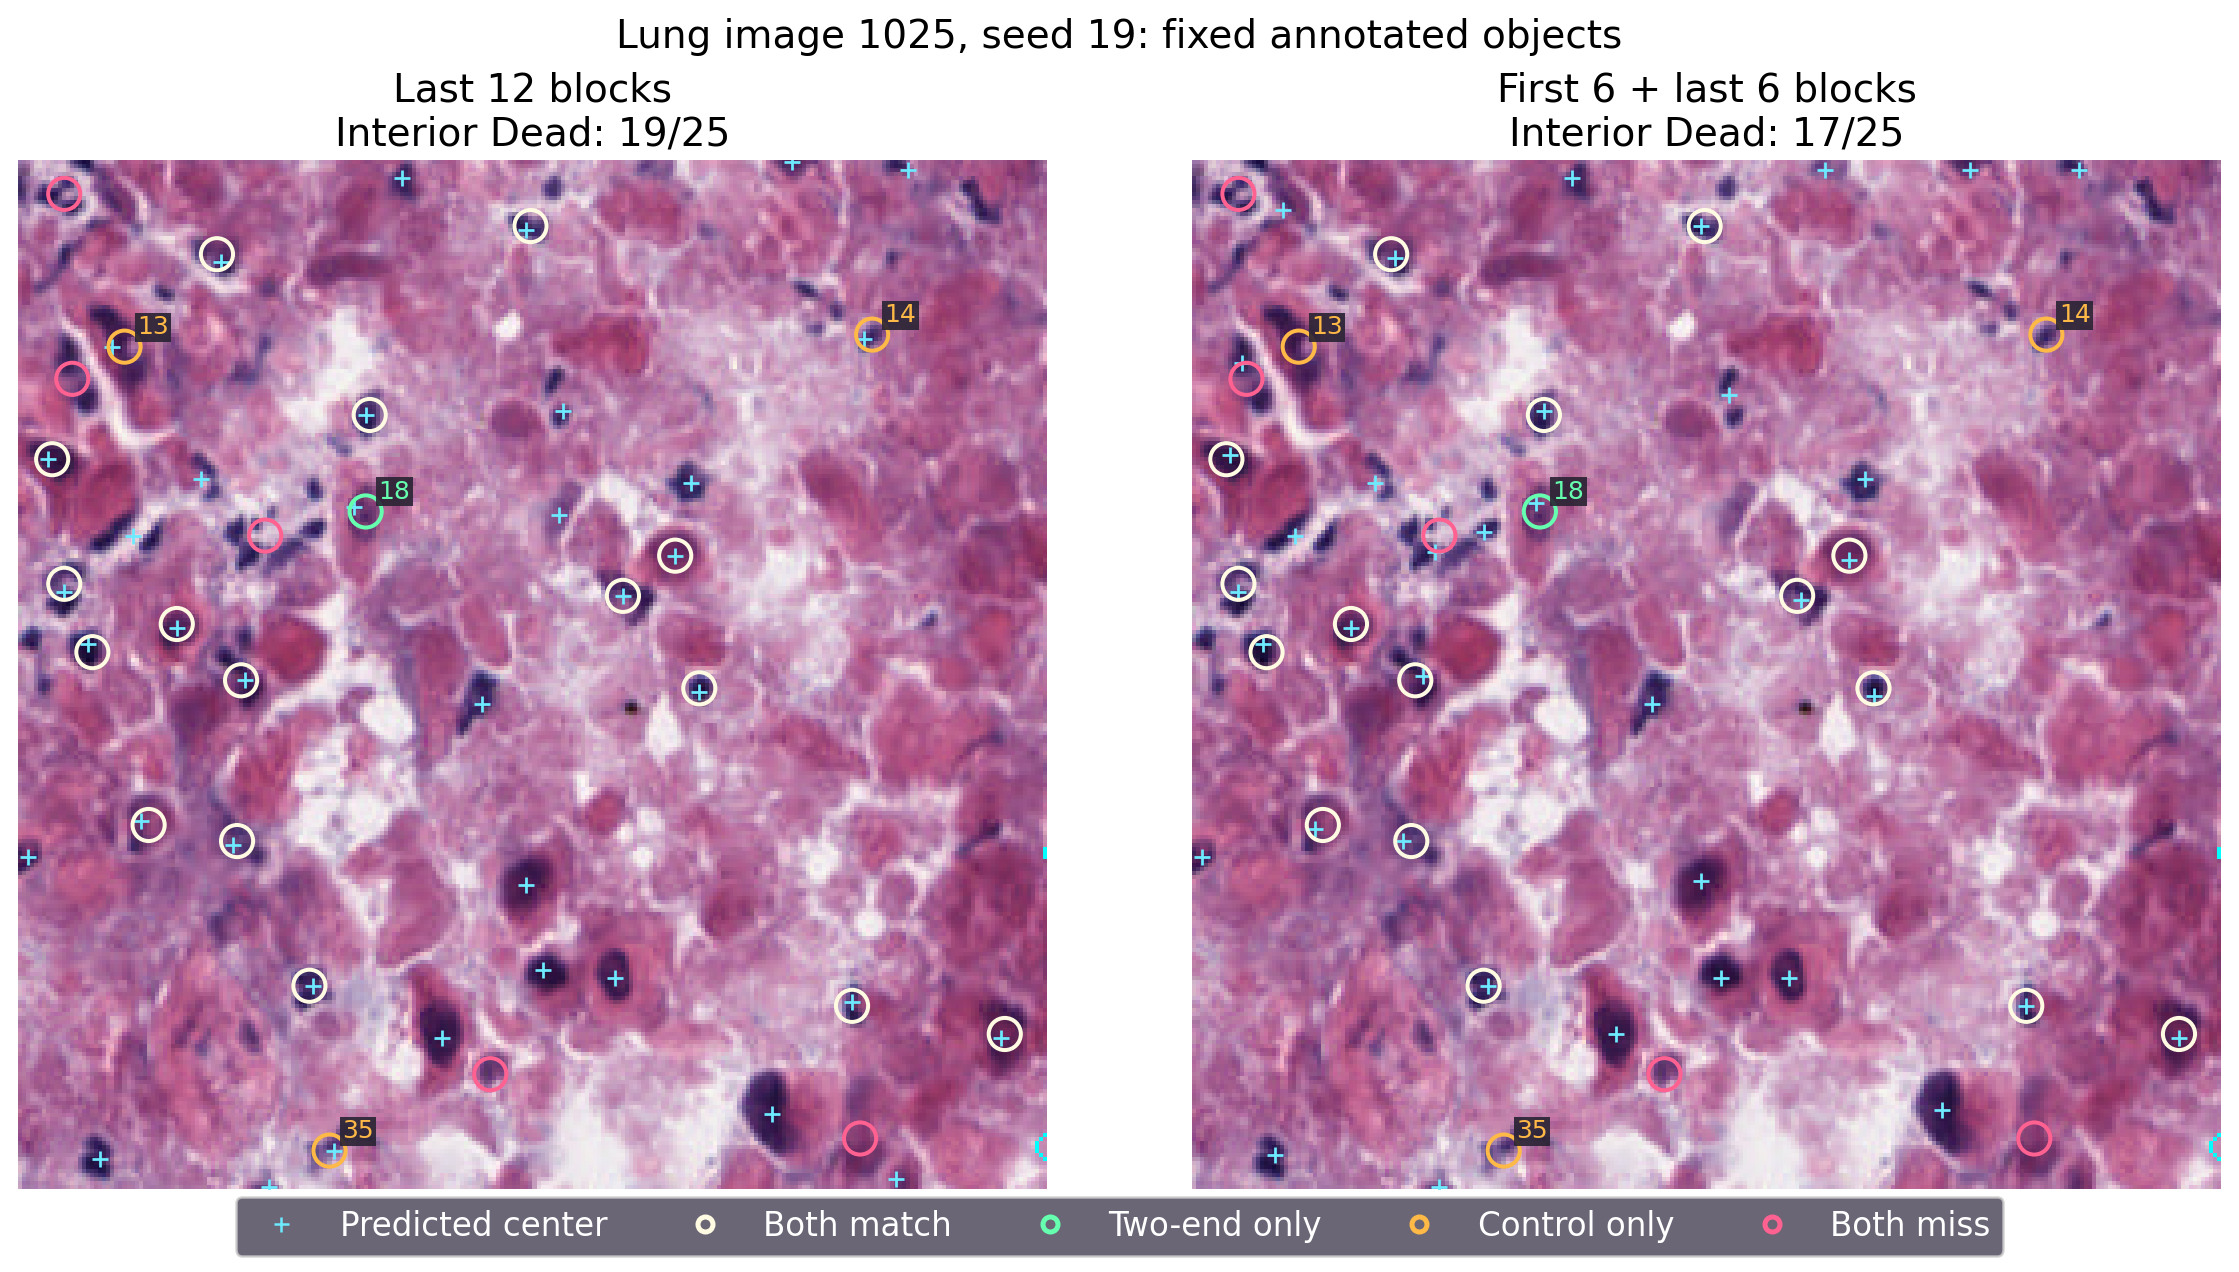
\includegraphics[width=\linewidth,height=0.40\textheight,keepaspectratio]{../figures/p29_image_1025_seed_19.png}
\captionof{figure}{肺组织图像 1025：新增与丢失同时发生}
\raggedright

肺组织图像 1025 从 19/25 降至 17/25。对象 18（87，86）的最近预测距离从 3.16 降至 2.24 像素，进入三像素匹配范围。对象 13（46，26）、对象 14（43，212）、对象 35（246，77）丢失匹配，距离分别从 3.00→14.56、2.24→41.77 和 1.00→18.36 像素。对象 14 面积仅 31 像素，视觉上也很小。实验模型在恢复一个对象的同时，失去了多个标注附近的有效输出；组织总量会掩盖这种交换。

\end{minipage}

\noindent

\begin{minipage}{\linewidth}\centering
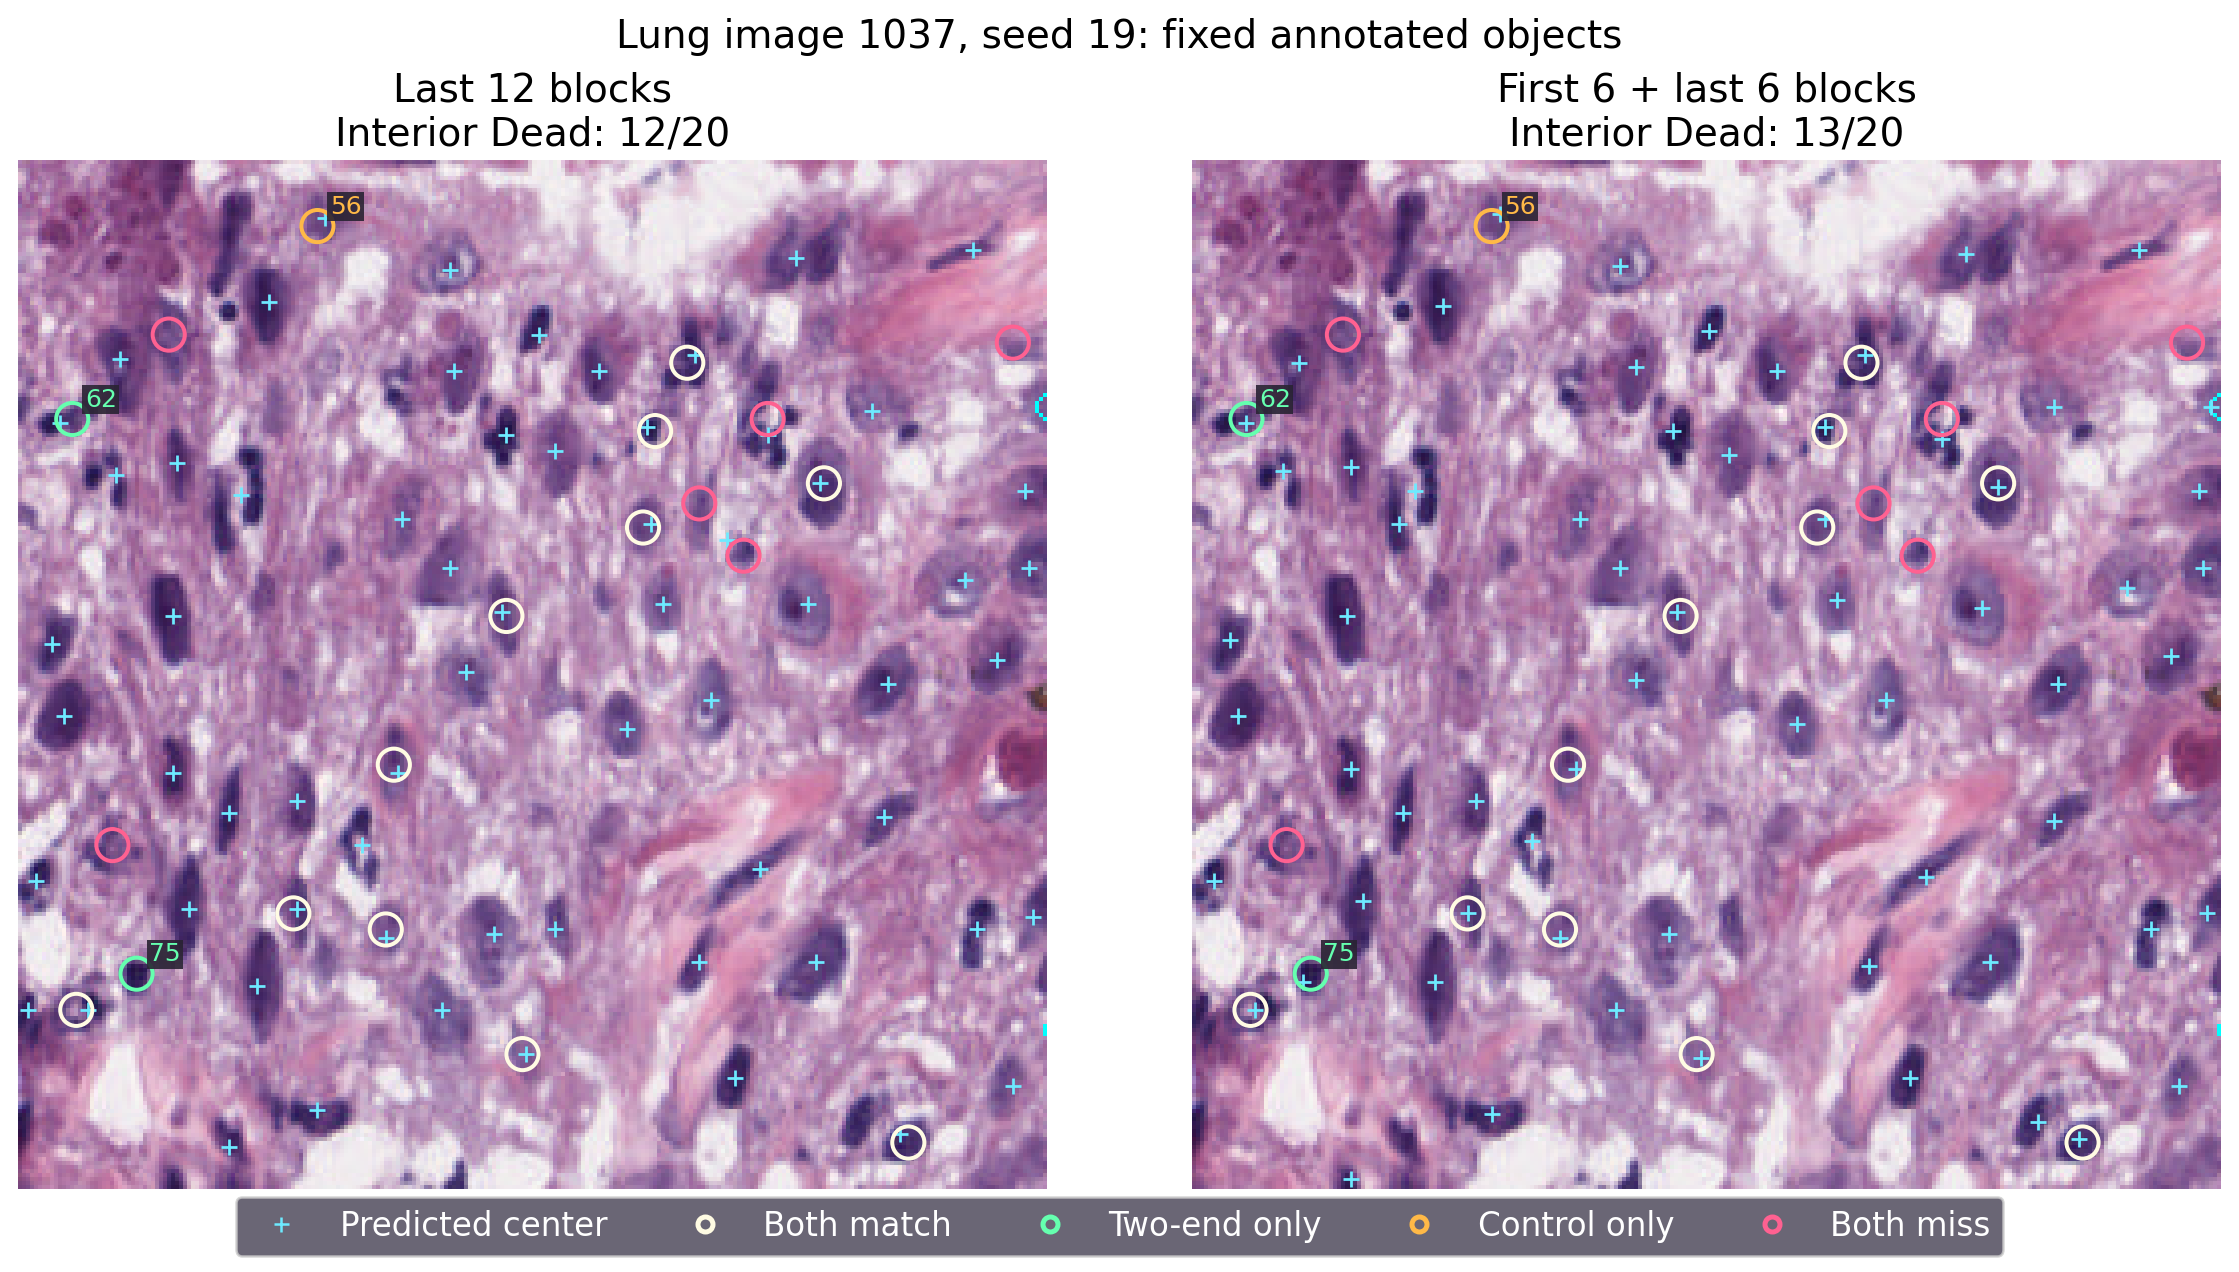
\includegraphics[width=\linewidth,height=0.40\textheight,keepaspectratio]{../figures/p29_image_1037_seed_19.png}
\captionof{figure}{肺组织图像 1037：小核恢复与匹配边界位移}
\raggedright

图像 1037 从 12/20 升至 13/20。对象 62（64，13）的距离从 3.16 降至 1.00 像素；面积 44 像素的对象 75（202，29）从 15.00 降至 2.83 像素，附近新增预测。对象 56（16，74）则因最近点从 2.83 移至 3.61 像素而失去匹配。前者表现为原来未覆盖邻域出现输出，后者表现为附近预测跨越固定匹配半径。

\end{minipage}

坐标记录确定了输出点的出现、消失和位移，原图提供染色、形态和组织环境。要把变化归因于中心分数、峰值抑制或编码器隐层，需要保存概率图或开展中间表征测量。本轮回收包含原图、标注中心、解码点和一对一匹配。

\subsection{种子
1：哪些改善在两个种子中一致}\label{ux79cdux5b50-1ux54eaux4e9bux6539ux5584ux5728ux4e24ux4e2aux79cdux5b50ux4e2dux4e00ux81f4}

\begin{longtable}[]{@{}
  >{\raggedright\arraybackslash}p{(\linewidth - 12\tabcolsep) * \real{0.1111}}
  >{\raggedleft\arraybackslash}p{(\linewidth - 12\tabcolsep) * \real{0.1481}}
  >{\raggedleft\arraybackslash}p{(\linewidth - 12\tabcolsep) * \real{0.1481}}
  >{\raggedleft\arraybackslash}p{(\linewidth - 12\tabcolsep) * \real{0.1481}}
  >{\raggedleft\arraybackslash}p{(\linewidth - 12\tabcolsep) * \real{0.1481}}
  >{\raggedleft\arraybackslash}p{(\linewidth - 12\tabcolsep) * \real{0.1481}}
  >{\raggedleft\arraybackslash}p{(\linewidth - 12\tabcolsep) * \real{0.1481}}@{}}
\toprule\noalign{}
\begin{minipage}[b]{\linewidth}\raggedright
种子 1 更新范围
\end{minipage} & \begin{minipage}[b]{\linewidth}\raggedleft
内部 Dead
\end{minipage} & \begin{minipage}[b]{\linewidth}\raggedleft
小 Dead
\end{minipage} & \begin{minipage}[b]{\linewidth}\raggedleft
全部匹配
\end{minipage} & \begin{minipage}[b]{\linewidth}\raggedleft
总召回
\end{minipage} & \begin{minipage}[b]{\linewidth}\raggedleft
精度
\end{minipage} & \begin{minipage}[b]{\linewidth}\raggedleft
未匹配预测
\end{minipage} \\
\midrule\noalign{}
\endhead
\bottomrule\noalign{}
\endlastfoot
最后十二层 & 67/145 & 7/32 & 7,329/12,250 & 59.83\% & 69.25\% & 3,255 \\
前六层＋后六层 & 80/145 & 11/32 & 7,494/12,250 & 61.18\% & 70.14\% &
3,191 \\
\end{longtable}

种子 1 多找到 13 个目标核，内部 Dead 召回增加 8.9655
个百分点，原固定重采样的 95\%
区间为［+3.1250，+20.4082］个百分点。实验模型多输出 101 个点、多匹配 165
个核。两个种子的总体召回、精度和小 Dead
覆盖均改善，训练集覆盖均下降；最终 Dead 召回和精度均未达到
0.60/0.75，原双种子完整条件为 false。两种子配对变化的描述性均值为 Dead
召回 +10.0 个百分点、总体召回 +1.83 个百分点、精度 +1.06
个百分点。两个种子使用相同图像，均值汇总重复训练结果，图像样本量保持原来的
522 张。

\begin{figure}[H]\centering
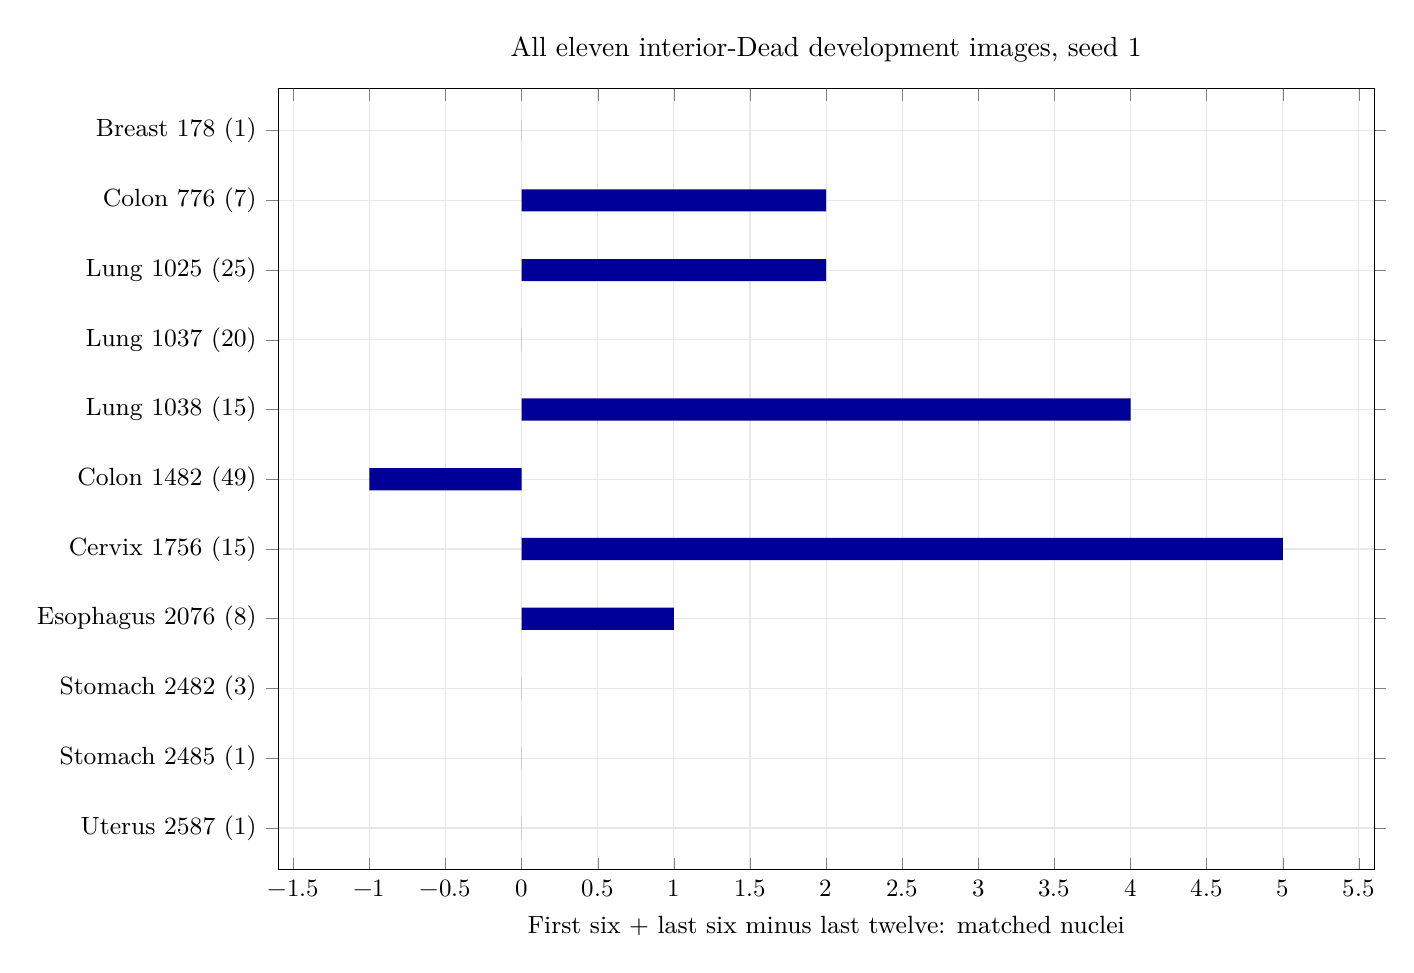
\begin{tikzpicture}
\begin{axis}[xbar,width=15.5cm,height=11.5cm,xlabel={First six + last six minus last twelve: matched nuclei},title={All eleven interior-Dead development images, seed 1},ytick={0,1,2,3,4,5,6,7,8,9,10},yticklabels={{Breast 178 (1)},{Colon 776 (7)},{Lung 1025 (25)},{Lung 1037 (20)},{Lung 1038 (15)},{Colon 1482 (49)},{Cervix 1756 (15)},{Esophagus 2076 (8)},{Stomach 2482 (3)},{Stomach 2485 (1)},{Uterus 2587 (1)}},ymin=-.6,ymax=10.6,y dir=reverse,bar width=8pt,grid=major,grid style={gray!18},tick label style={font=\small},label style={font=\small},title style={font=\normalsize}]
\addplot[fill=blue!60!black,draw=none] coordinates {(0,0) (2,1) (2,2) (0,3) (4,4) (-1,5) (5,6) (1,7) (0,8) (0,9) (0,10)};
\end{axis}
\end{tikzpicture}

\caption{种子 1 的全部目标阳性图像}
\end{figure}

种子 1 有五张图像增加、一张减少、五张不变。肺组织贡献 +6，宫颈 +5，结肠
+1，食管 +1。肺组织图像 1038 在种子 19/1 中分别增加 5/4 个；宫颈图像
1756 增加 2/5 个。结肠图像 1482 则分别为 13/49→13/49 和
11/49→10/49，仍遗漏 36/39 个目标核。肺组织图像 1025
在两个种子中的净变化为
−2/+2。总体改善同方向，贡献图像与具体对象却有差异。种子 1
逐一去掉一张阳性图像后，改善仍为 +6.15～+14.58 个百分点；种子 19 为
+8.03～+16.67 个百分点。

\begin{figure}[H]\centering
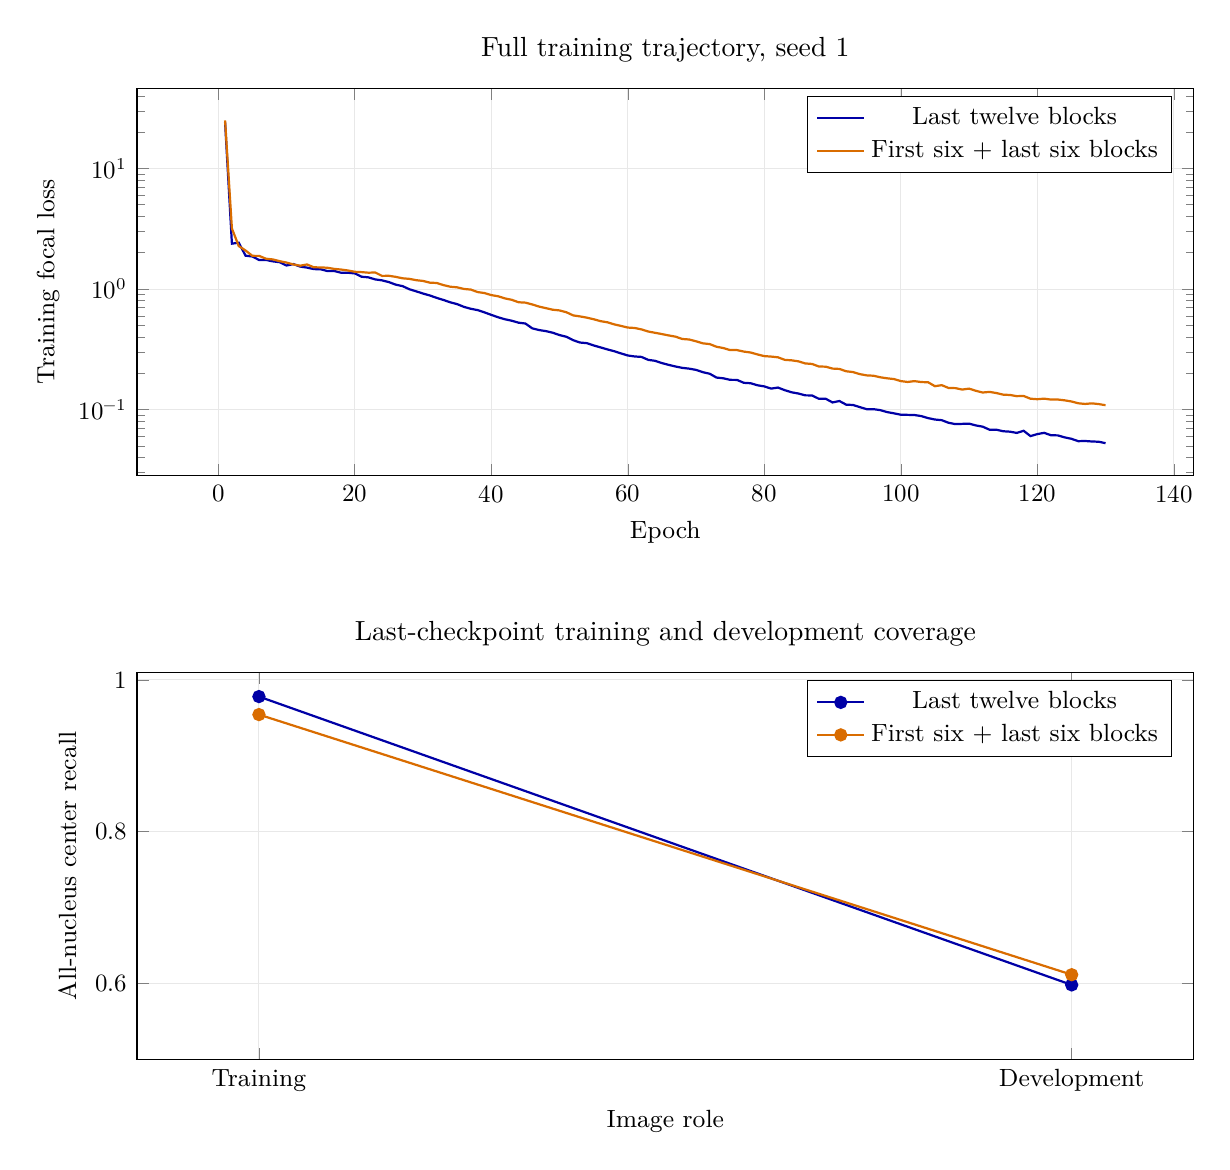
\begin{tikzpicture}
\begin{groupplot}[group style={group size=1 by 2,vertical sep=2.5cm},width=15cm,height=6.5cm,grid=major,grid style={gray!18},legend style={font=\small},tick label style={font=\small},label style={font=\small},title style={font=\normalsize}]
\nextgroupplot[xlabel={Epoch},ylabel={Training focal loss},ymode=log,title={Full training trajectory, seed 1}]
\addplot[thick,color=blue!65!black] coordinates {(1,24.1464097734) (2,2.37907460558) (3,2.42395087085) (4,1.89138898435) (5,1.86317232623) (6,1.74016351449) (7,1.74304416577) (8,1.69685451805) (9,1.67006233835) (10,1.56766110955) (11,1.61067377605) (12,1.53629610102) (13,1.50642142742) (14,1.46387814283) (15,1.45853354044) (16,1.41012065469) (17,1.41155984639) (18,1.36500526315) (19,1.36530261288) (20,1.34831311802) (21,1.26601811308) (22,1.25017444218) (23,1.20228692476) (24,1.18028517604) (25,1.1418605139) (26,1.08759826323) (27,1.05754919494) (28,0.996463930121) (29,0.957315703475) (30,0.917854604012) (31,0.884611722316) (32,0.844783207316) (33,0.811727376824) (34,0.776253122491) (35,0.749918353982) (36,0.711522315581) (37,0.686212550342) (38,0.669188185367) (39,0.640575755677) (40,0.610953438793) (41,0.583465234451) (42,0.561700555565) (43,0.546217831615) (44,0.526078422094) (45,0.517960491947) (46,0.472479875761) (47,0.457218615077) (48,0.447917287302) (49,0.434525593117) (50,0.415261976218) (51,0.402127236924) (52,0.376605498303) (53,0.36019223948) (54,0.35605725737) (55,0.340845657169) (56,0.328337270135) (57,0.315999150119) (58,0.305300156355) (59,0.292695673722) (60,0.281272957718) (61,0.276108612035) (62,0.273762871861) (63,0.258717186539) (64,0.25410910973) (65,0.243317074278) (66,0.235023784918) (67,0.227832109364) (68,0.222026201752) (69,0.218754308852) (70,0.213573085317) (71,0.204481938093) (72,0.198484528042) (73,0.184561390548) (74,0.181954261069) (75,0.176659237433) (76,0.176465889512) (77,0.166919391089) (78,0.165605806076) (79,0.159267719343) (80,0.155895322193) (81,0.149444878387) (82,0.152472293931) (83,0.145000228475) (84,0.13933104506) (85,0.136019747531) (86,0.131397780628) (87,0.131108616685) (88,0.122979612943) (89,0.123099924053) (90,0.114715974734) (91,0.117932853594) (92,0.109995811722) (93,0.10931592318) (94,0.104908588645) (95,0.100949496105) (96,0.100945127414) (97,0.0990364957451) (98,0.0954205769698) (99,0.0931880944945) (100,0.0907757309053) (101,0.0905180393667) (102,0.0902303193452) (103,0.088424334828) (104,0.0850573193147) (105,0.0828130932458) (106,0.0817788428467) (107,0.0778135305542) (108,0.0758810507128) (109,0.076215800676) (110,0.0765656325285) (111,0.073964573264) (112,0.0722589833385) (113,0.0681890490755) (114,0.0681911942967) (115,0.0661841659039) (116,0.0656570426451) (117,0.0641314384799) (118,0.0668080432189) (119,0.0603444048726) (120,0.0626898991414) (121,0.0642267048966) (122,0.0613357394715) (123,0.0611648887737) (124,0.0588851603053) (125,0.0573119477154) (126,0.0547676310772) (127,0.0549531287133) (128,0.0544491219801) (129,0.0541878870772) (130,0.052713020613)};
\addlegendentry{Last twelve blocks}
\addplot[thick,color=orange!85!black] coordinates {(1,25.011496911) (2,3.17799959623) (3,2.27436188492) (4,2.08865700683) (5,1.885834561) (6,1.8839197844) (7,1.78421891875) (8,1.76084290541) (9,1.70301685874) (10,1.65851540155) (11,1.59998793002) (12,1.56235476789) (13,1.59959509592) (14,1.51503495644) (15,1.51149311659) (16,1.50238437958) (17,1.4696641211) (18,1.45096074566) (19,1.42595314957) (20,1.39012699037) (21,1.38180783916) (22,1.36672399956) (23,1.37209300751) (24,1.28553308058) (25,1.28794003566) (26,1.26253414447) (27,1.22821307152) (28,1.21486726833) (29,1.18446103696) (30,1.16763180768) (31,1.12988207348) (32,1.12319189014) (33,1.07810610866) (34,1.04555361918) (35,1.033199504) (36,1.00191194403) (37,0.990080934014) (38,0.944060752715) (39,0.926574528371) (40,0.891300759756) (41,0.871630537951) (42,0.836584058926) (43,0.81430716645) (44,0.77721205911) (45,0.771726598473) (46,0.745692780707) (47,0.715607827831) (48,0.694585677345) (49,0.67398442983) (50,0.665043073873) (51,0.64224857131) (52,0.604723203274) (53,0.593133849232) (54,0.579252798606) (55,0.562060371949) (56,0.541903383772) (57,0.530444192252) (58,0.509721531137) (59,0.494748991699) (60,0.47940543766) (61,0.475636233514) (62,0.462900746059) (63,0.444441580239) (64,0.43372605681) (65,0.423428376604) (66,0.412513215189) (67,0.402878855115) (68,0.385366324147) (69,0.381752724151) (70,0.368892222992) (71,0.354728576386) (72,0.34968104504) (73,0.332328972624) (74,0.324155154326) (75,0.311755497574) (76,0.311781367654) (77,0.303075165604) (78,0.297676424355) (79,0.287003625485) (80,0.277921598474) (81,0.275451032265) (82,0.271752992647) (83,0.25877414053) (84,0.256390396781) (85,0.251566645488) (86,0.241655978028) (87,0.239265075389) (88,0.227968502746) (89,0.227136093183) (90,0.218998449615) (91,0.217567150648) (92,0.208101390862) (93,0.204921622139) (94,0.196992543635) (95,0.192389015248) (96,0.19113709086) (97,0.185506416595) (98,0.181884586101) (99,0.17933309276) (100,0.172520445635) (101,0.16965263944) (102,0.172393440965) (103,0.169369802517) (104,0.168656573035) (105,0.156491421992) (106,0.159630250606) (107,0.151222903264) (108,0.150808054505) (109,0.146756133286) (110,0.149384039095) (111,0.143327694706) (112,0.138696835582) (113,0.140289669869) (114,0.137317749343) (115,0.133153271166) (116,0.132303883946) (117,0.129376130577) (118,0.129833591042) (119,0.123228266547) (120,0.122043808987) (121,0.123365918834) (122,0.121185603338) (123,0.121300019186) (124,0.119477846619) (125,0.116899685834) (126,0.112925518259) (127,0.111518024011) (128,0.112746420551) (129,0.11120598165) (130,0.108816306706)};
\addlegendentry{First six + last six blocks}
\nextgroupplot[xlabel={Image role},ylabel={All-nucleus center recall},title={Last-checkpoint training and development coverage},xtick={0,1},xticklabels={Training,Development},xmin=-.15,xmax=1.15,ymin=.5,ymax=1.01]
\addplot[thick,mark=*,color=blue!65!black] coordinates {(0,0.978025427719) (1,0.598285714286)};
\addlegendentry{Last twelve blocks}
\addplot[thick,mark=*,color=orange!85!black] coordinates {(0,0.954324281902) (1,0.611755102041)};
\addlegendentry{First six + last six blocks}
\end{groupplot}
\end{tikzpicture}

\caption{种子 1 的训练过程与开发评估覆盖}
\end{figure}

训练集总体召回从 97.80\% 降至 95.43\%，内部 Dead 匹配从 624/656 降至
606/656。记录的训练时间为 4.0143/6.7220 小时，检查点写入时间为
238.77/2,116.75 秒，实验模型完成训练和评估的应用总耗时为 10.1409
小时。种子 1 实验模型经历了长时间 Lustre
延迟，这些耗时包含等待，用于记录实际资源成本；种子 19 的 21.24\%
训练时间增加更适合描述本轮更新范围的常规成本差异。两种子的训练峰值已分配显存均约为
4.05/4.84 GiB。

\subsection{固定对象：重复恢复、重复丢失与相互抵消}\label{ux56faux5b9aux5bf9ux8c61ux91cdux590dux6062ux590dux91cdux590dux4e22ux5931ux4e0eux76f8ux4e92ux62b5ux6d88}

种子 1 的八张固定样例共同找到 29 个、新增 7 个、丢失 3 个、共同漏检 14
个，53 个目标对象净增加 4 个；种子 19 分别为 30、6、4、13，净增加 2
个。以下分析沿用相同标注编号和原始坐标。

\noindent

\begin{minipage}{\linewidth}\centering
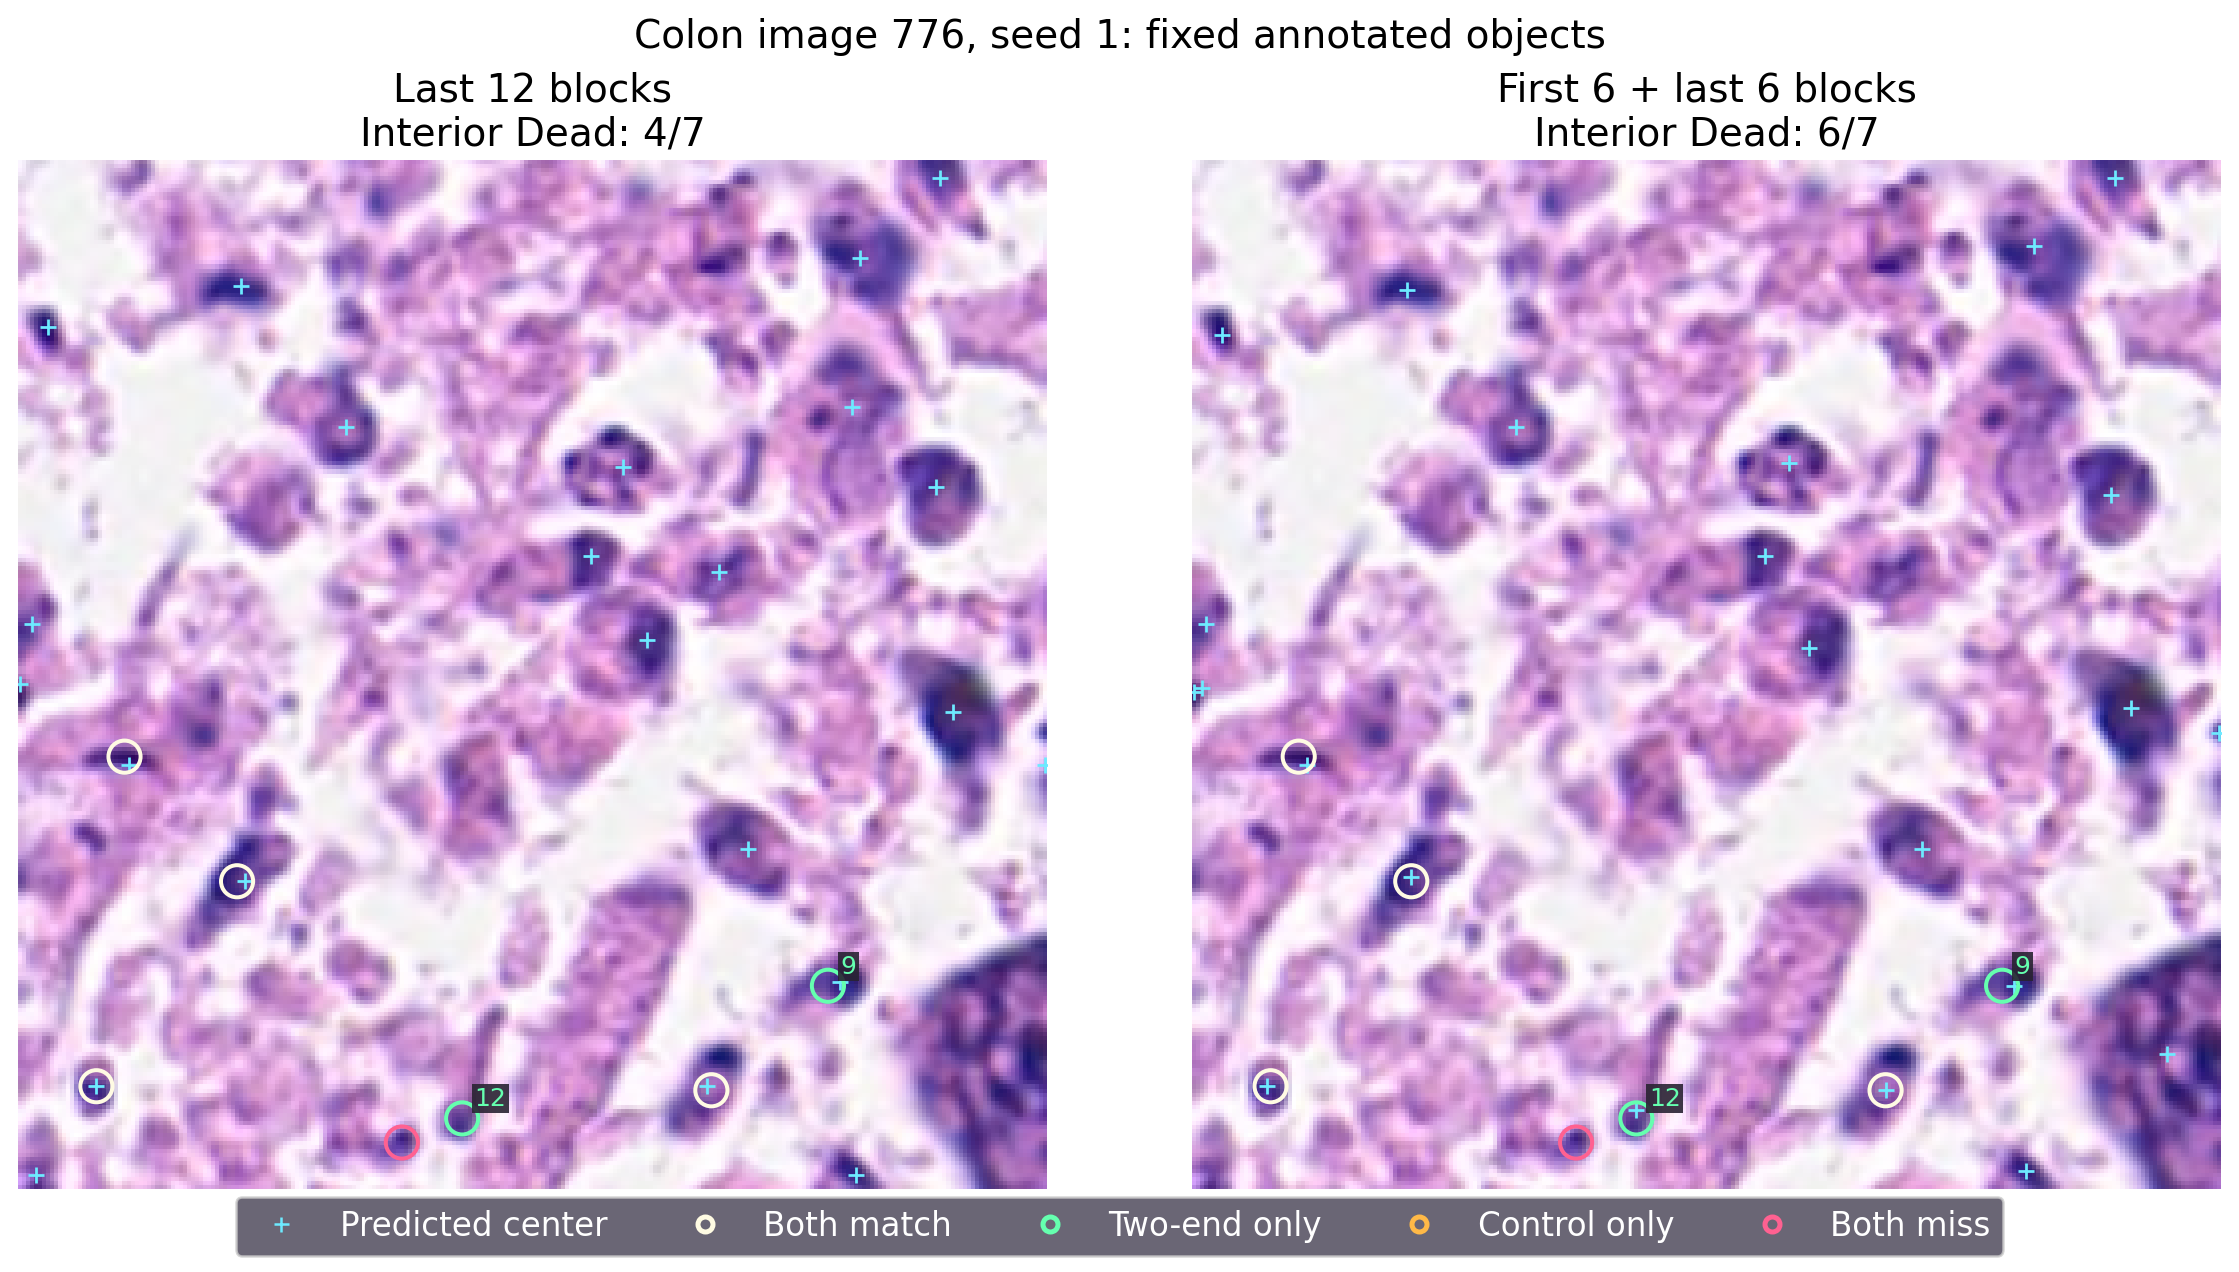
\includegraphics[width=\linewidth,height=0.40\textheight,keepaspectratio]{../figures/p29_image_776_seed_1.png}
\captionof{figure}{种子 1 的结肠图像 776}
\raggedright

结肠图像 776 从 4/7 增至 6/7。对象 12 位于（238，110），面积为 104 像素，在两个种子中均被找回：最近点距离在种子 19 为 80.66→1.00，种子 1 为 61.52→2.00 像素。这是在同一个标注上重复观察到的恢复。种子 1 还找回对象 9（205，201），面积 191，距离从 3.16 降至 3.00 像素；种子 19 则找回下方组织带中的对象 10 和 11。相似的图像总改善可以来自不同细胞核。

\end{minipage}

\noindent

\begin{minipage}{\linewidth}\centering
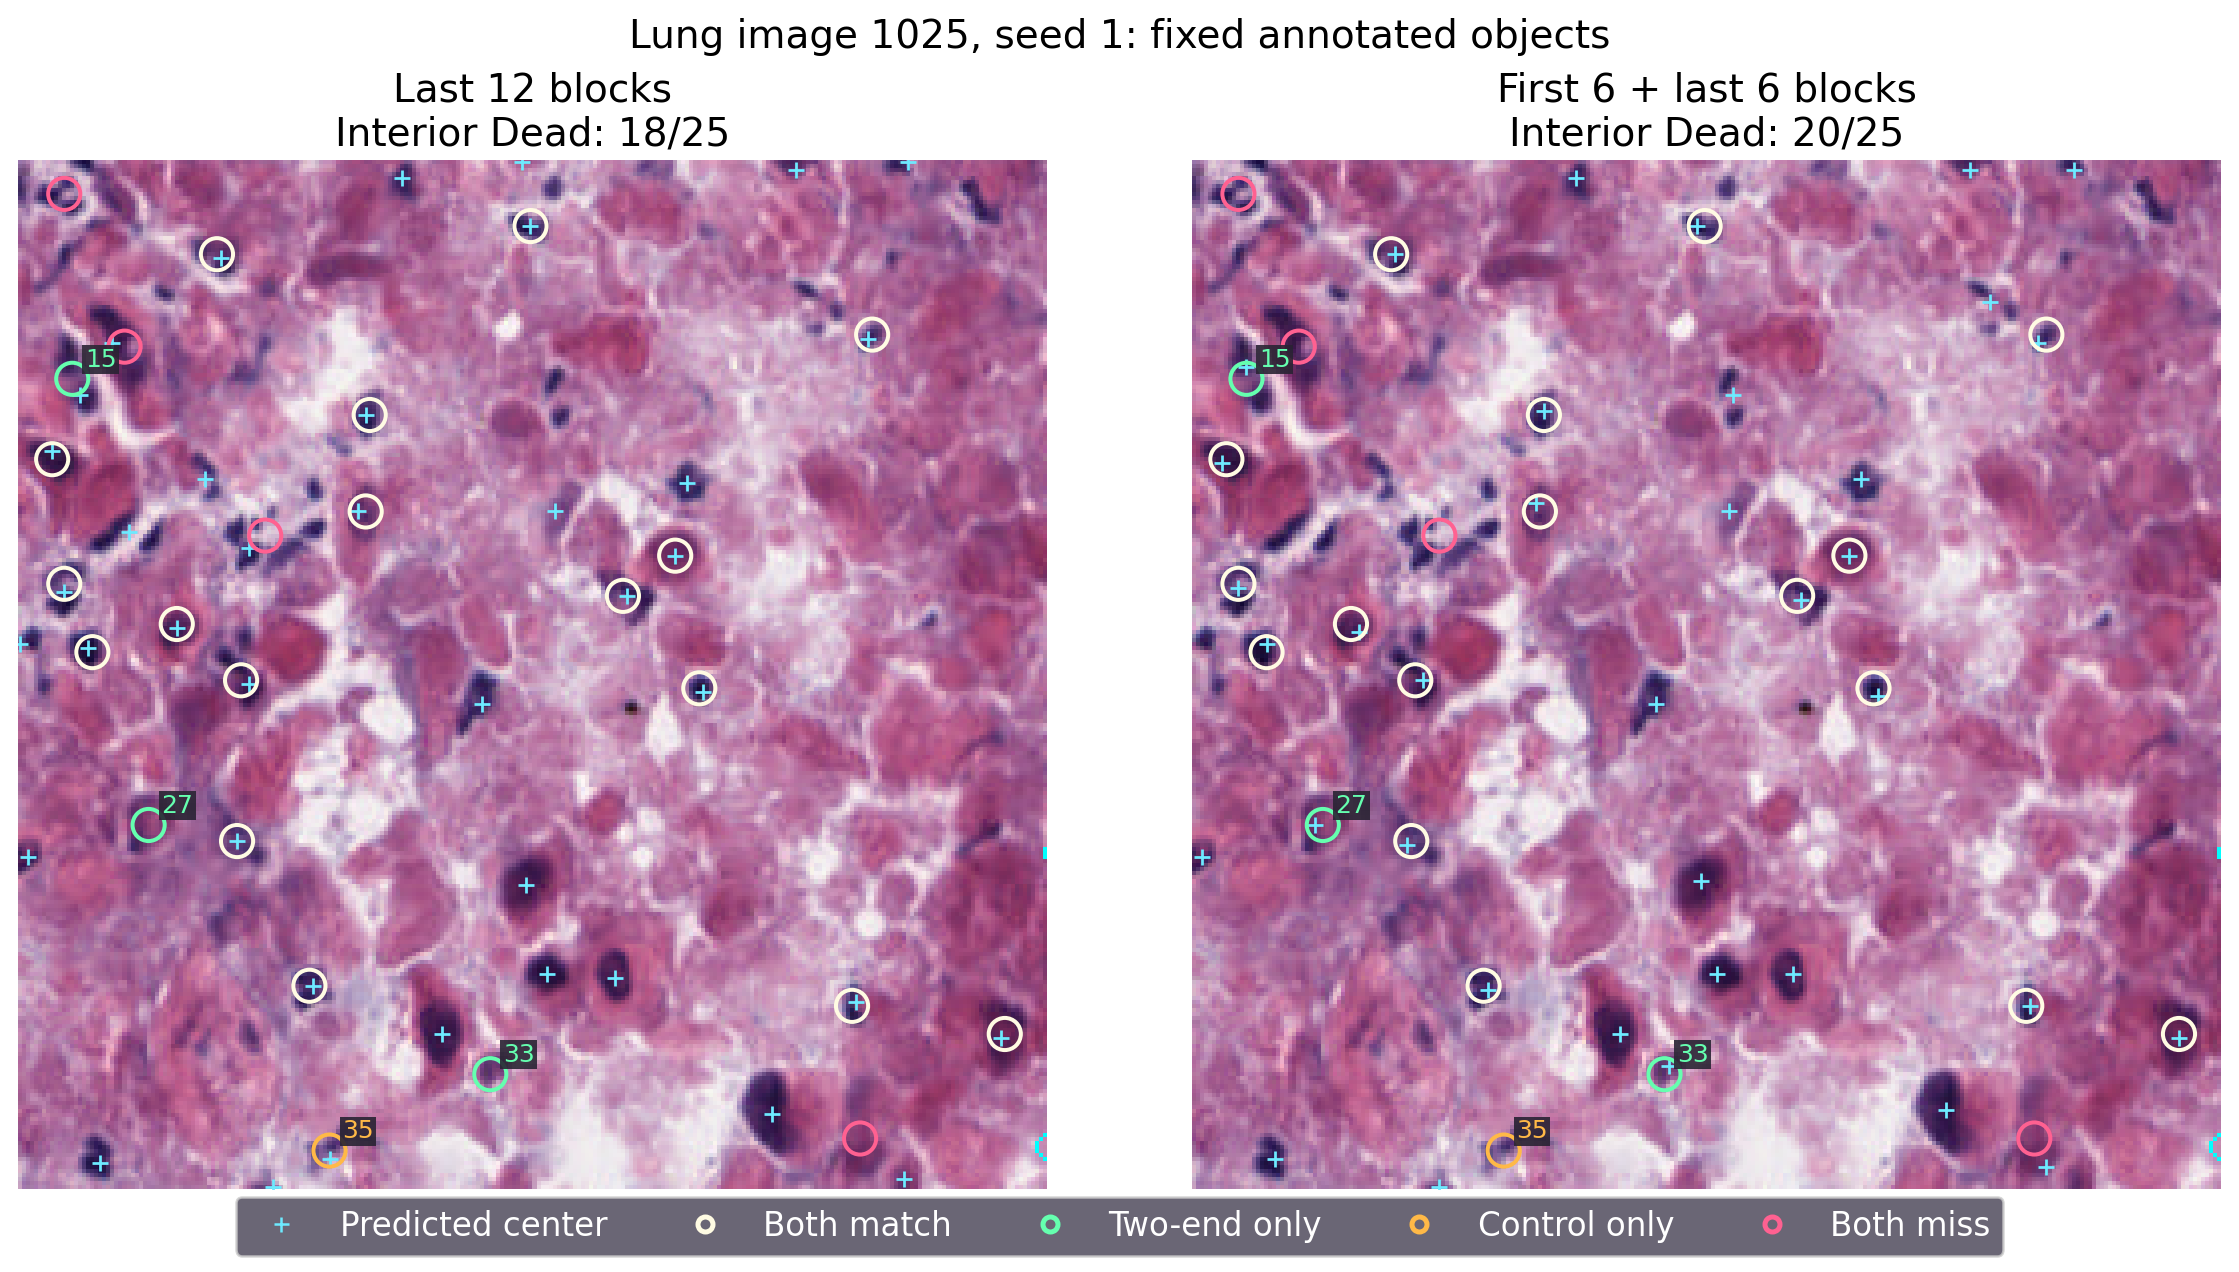
\includegraphics[width=\linewidth,height=0.40\textheight,keepaspectratio]{../figures/p29_image_1025_seed_1.png}
\captionof{figure}{种子 1 的肺组织图像 1025}
\raggedright

图像 1025 从 18/25 增至 20/25。对象 15（54，13）、27（165，32）、33（227，117）新增匹配，距离分别为 4.47→3.00、22.36→2.00、15.62→2.24 像素。对象 33 面积 52，属于预定义的小核组。对象 35（246，77）面积 68，在两个种子中均丢失：种子 19 为 1.00→18.36，种子 1 为 2.00→18.36 像素。重复出现的局部丢失与肺组织总量的改善同时存在。

\end{minipage}

\noindent

\begin{minipage}{\linewidth}\centering
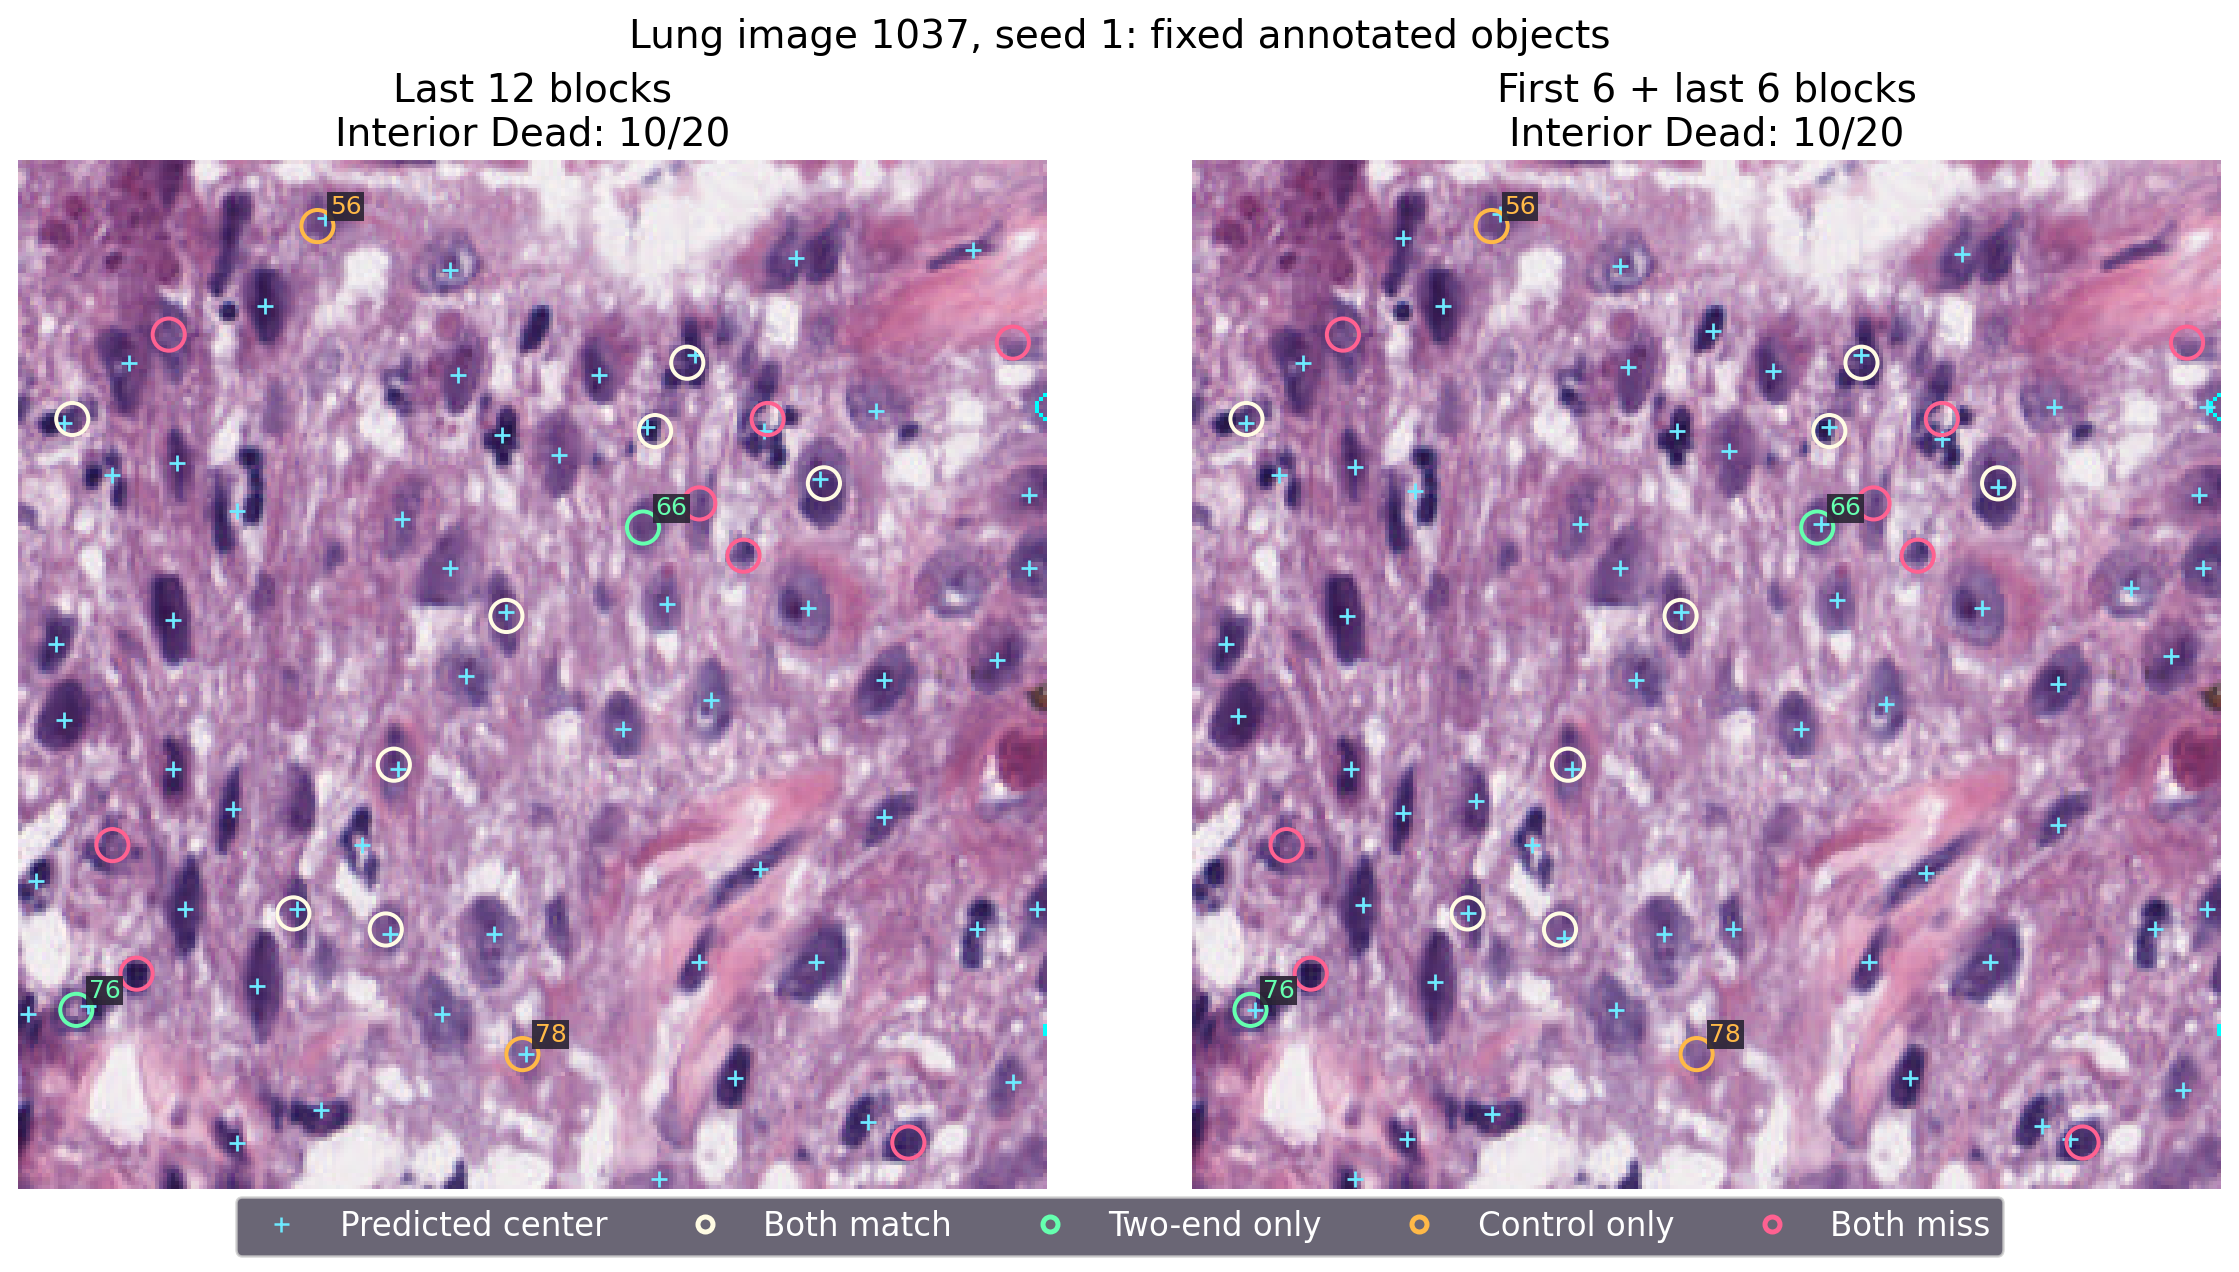
\includegraphics[width=\linewidth,height=0.40\textheight,keepaspectratio]{../figures/p29_image_1037_seed_1.png}
\captionof{figure}{种子 1 的肺组织图像 1037}
\raggedright

图像 1037 保持 10/20，但内部发生两个新增和两个丢失。对象 66（91，155）、76（211，14）距离为 19.92→1.41 和 3.16→1.00；对象 56（16，74）、78（222，125）距离为 2.83→3.61 和 1.00→22.83 像素。对象 56 在两个种子中跨越了完全相同的匹配边界。因此，图像匹配数不变也可能包含重复的定位丢失，以及其他核的补偿恢复。全部逐核距离、预测中心和一对一分配均保存在坐标 JSON 与 CSV 中。

\end{minipage}

\subsection{下一轮与保存记录}\label{ux4e0bux4e00ux8f6eux4e0eux4fddux5b58ux8bb0ux5f55}

P30 固定更新中间十二层，补齐连续层位置比较，保留 151,179,264
个编码器可训练参数、3,294,657 个检测头参数、原学习率、130
轮、种子、数据和判定。GPU
验收需证明梯度能通过冻结的后续层到达中间层，并且冻结参数保持不变。它属于适应性的开发实验，结果将按原规则完整报告。

合并后的科学结果包记录并核验了 92 个小产物的 SHA256，其中含 48 张最终
PNG；505 个源码文件的校验沿用此前已核验的种子 19 回收。种子 19
和对照种子 1 的小产物与原保存清单相符。实验种子 1
在模型完成后的保存阶段超时；随后 CPU 恢复作业 55745860 用 185
秒保存了全部 23 个文件，包括两个检查点和 12 张最终
PNG，并对源文件和目标回读分别计算哈希。21
个小文件与先前回收完全一致。其余六个检查点大小与原清单相符，六者独立重哈希及外部归档仍待安排。\href{../P29_PRESERVATION_RECOVERY.json}{保存恢复记录}
提供已核验的检查点哈希。\href{../p29_verified_analysis.json}{完整数值分析}、\href{../object_summary.json}{对象变化}、\href{../stage_pairs.csv}{阶段成对表}
和 \href{../collection_result.json}{回收核验}
随报告保存。原双种子完整条件均未通过，按原规则关闭这一前六层加后六层设置；其一致的配对改善为已独立冻结的中间十二层比较提供了研究依据。

\end{document}
